%% LyX 1.3 created this file.  For more info, see http://www.lyx.org/.
%% Do not edit unless you really know what you are doing.
\documentclass[english]{article}
\usepackage[T1]{fontenc}
\usepackage[latin1]{inputenc}
\usepackage{geometry}
\geometry{verbose,letterpaper,tmargin=1in,bmargin=1in,lmargin=1in,rmargin=1in}
\usepackage{verbatim}
\usepackage{subfigure}
\usepackage{graphicx}
\usepackage{amssymb}
\IfFileExists{url.sty}{\usepackage{url}}
                      {\newcommand{\url}{\texttt}}

\makeatletter

%%%%%%%%%%%%%%%%%%%%%%%%%%%%%% LyX specific LaTeX commands.
%% Bold symbol macro for standard LaTeX users
\providecommand{\boldsymbol}[1]{\mbox{\boldmath $#1$}}

%% Because html converters don't know tabularnewline
\providecommand{\tabularnewline}{\\}

\usepackage{babel}
\makeatother
\begin{document}

\title{SciPy Tutorial}


\author{Travis E. Oliphant}

\maketitle

\section{Introduction}

SciPy is a collection of mathematical algorithms and convenience functions
built on the Numeric extension for Python. It adds significant power
to the interactive Python session by exposing the user to high-level
commands and classes for the manipulation and visualization of data.
With SciPy, an interactive Python session becomes a data-processing
and system-prototyping environment rivaling sytems such as Matlab,
IDL, Octave, R-Lab, and SciLab. 

The additional power of using SciPy within Python, however, is that
a powerful programming language is also available for use in developing
sophisticated programs and specialized applications. Scientific applications
written in SciPy benefit from the development of additional modules
in numerous niche's of the software landscape by developers across
the world. Everything from parallel programming to web and data-base
subroutines and classes have been made available to the Python programmer.
All of this power is available in addition to the mathematical libraries
in SciPy.

This document provides a tutorial for the first-time user of SciPy
to help get started with some of the features available in this powerful
package. It is assumed that the user has already installed the package.
Some general Python facility is also assumed such as could be acquired
by working through the Tutorial in the Python distribution. Throughout
this tutorial it is assumed that the user has imported all of the
names defined in the SciPy namespace using the command \begin{verbatim}
>>> from scipy import *\end{verbatim} 


\subsection{General Help}

Python provides the facility of documentation strings. The functions
and classes available in SciPy use this method for on-line documentation.
There are two methods for reading these messages and getting help.
Python provides the command \textbf{help} in the pydoc module. Entering
this command with no arguments (i.e. >\,{}>\,{}>
help ) launches an interactive help session that allows searching
through the keywords and modules available to all of Python. Running
the command help with an object as the argument displays the calling
signature, and the documentation string of the object.

The pydoc method of help is sophisticated but uses a pager to display
the text. Sometimes this can interfere with the terminal you are running
the interactive session within. A scipy-specific help system is also
available under the command scipy.info. The signature and documentation
string for the object passed to the help command are printed to standard
output (or to a writeable object passed as the third argument). The
second keyword argument of {}``scipy.info'' defines the maximum
width of the line for printing. If a module is passed as the argument
to help than a list of the functions and classes defined in that module
is printed. For example:

\verbatiminput{example1.1}

Another useful command is \textbf{source.} When given a function written
in Python as an argument, it prints out a listing of the source code
for that function. This can be helpful in learning about an algorithm
or understanding exactly what a function is doing with its arguments.
Also don't forget about the Python command \texttt{dir} which can
be used to look at the namespace of a module or package.


\subsection{SciPy Organization}

SciPy is organized into subpackages covering different scientific
computing domains. Some common functions which several subpackages
rely on live under the \texttt{scipy\_base} package which is installed
at the same directory level as the scipy package itself and could
be installed separately. This allows for the possibility of separately
distributing the subpackages of scipy as long as scipy\_base package
is provided as well. 

Two other packages are installed at the higher-level: scipy\_distutils
and weave. These two packages while distributed with main scipy package
could see use independently of scipy and so are treated as separate
packages and described elsewhere.

The remaining subpackages are summarized in the following table (a
{*} denotes an optional sub-package that requires additional libraries
to function or is not available on all platforms). 

\begin{center}\begin{tabular}{|c|c|}
\hline 
Subpackage&
Description\tabularnewline
\hline
\hline 
cluster&
Clustering algorithms\tabularnewline
\hline 
cow&
Cluster of Workstations code for parallel programming\tabularnewline
\hline 
fftpack&
FFT based on fftpack -- default\tabularnewline
\hline 
fftw{*}&
FFT based on fftw --- requires FFTW libraries (is this still needed?)\tabularnewline
\hline 
ga&
Genetic algorithms\tabularnewline
\hline 
gplt{*}&
Plotting --- requires gnuplot\tabularnewline
\hline 
integrate&
Integration\tabularnewline
\hline 
interpolate&
Interpolation\tabularnewline
\hline 
io&
Input and Output\tabularnewline
\hline 
linalg&
Linear algebra\tabularnewline
\hline 
optimize&
Optimization and root-finding routines\tabularnewline
\hline 
plt{*}&
Plotting --- requires wxPython\tabularnewline
\hline 
signal&
Signal processing\tabularnewline
\hline 
special&
Special functions\tabularnewline
\hline 
stats&
Statistical distributions and functions\tabularnewline
\hline 
xplt&
Plotting with gist\tabularnewline
\hline
\end{tabular}\end{center}

Because of their ubiquitousness, some of the functions in these subpackages
are also made available in the scipy namespace to ease their use in
interactive sessions and programs. In addition, many convenience functions
are located in the scipy\_base package and the in the top-level of
the scipy package. Before looking at the sub-packages individually,
we will first look at some of these common functions. 


\section{Basic functions in scipy\_base and top-level scipy}


\subsection{Interaction with Numeric}

To begin with, all of the Numeric functions have been subsumed into
the scipy namespace so that all of those functions are available without
additionally importing Numeric. In addition, the universal functions
(addition, subtraction, division) have been altered to not raise exceptions
if floating-point errors are encountered%
\footnote{These changes are all made in a new module (fastumath) that is part
of the scipy\_base package. The old functionality is still available
in umath (part of Numeric) if you need it (note: importing umath or
fastumath resets the behavior of the infix operators to use the umath
or fastumath ufuncs respectively). %
}, instead NaN's and Inf's are returned in the arrays. To assist in
detection of these events new universal functions (isnan, isfinite,
isinf) have been added. In addition, the comparision operators have
been changed to allow comparisons and logical operations of complex
numbers (only the real part is compared). Also, with the new universal
functions in SciPy, the logical operations (except logical\_XXX functions)
all return arrays of unsigned bytes (8-bits per element instead of
the old 32-bits, or even 64-bits) per element%
\footnote{Be careful when treating logical expressions as integers as the 8-bit
integers may silently overflow at 256.%
}. 

Finally, some of the basic functions like log, sqrt, and inverse trig
functions have been modified to return complex numbers instead of
NaN's where appropriate (\emph{i.e.} \texttt{scipy.sqrt(-1)} returns
\texttt{1j}). 


\subsection{Alter numeric}

With the command \textbf{scipy.alter\_numeric()} you can now use index
and mask arrays inside brackets and the coercion rules of Numeric
are changed so that Python scalars will not upcast the results of
operations. An example is shown below 


\subsection{Scipy\_base routines }

The purpose of scipy\_base is to collect general-purpose routines
that the other sub-packages can use. These routines are divided into
several files for organizational purposes, but they are all available
under the scipy\_base namespace (and the scipy namespace). There are
routines for type handling and type checking, shape and matrix manipulation,
polynomial processing, and other useful functions. Rather than giving
a detailed description of each of these functions (which is available
using the \textbf{help}, \textbf{info} and \textbf{source} commands),
this tutorial will discuss some of the more useful commands which
require a little introduction to use to their full potential. 


\subsubsection{Type handling }

Note the difference between \textbf{iscomplex} (\textbf{isreal}) and
\textbf{iscomplexobj} (\textbf{isrealobj}). The former command is
array based and returns byte arrays of ones and zeros providing the
result of the element-wise test. The latter command is object based
and returns a scalar describing the result of the test on the entire
object. 

Often it is required to get just the real and/or imaginary part of
a complex number. While complex numbers and arrays have attributes
that return those values, if one is not sure whether or not the object
will be complex-valued, it is better to use the functional forms \textbf{real}
and \textbf{imag}. These functions succeed for anything that can be
turned into a Numeric array. Consider also the function \textbf{real\_if\_close}
which transforms a complex-valued number with tiny imaginary part
into a real number. 

Occasionally the need to check whether or not a number is a scalar
(Python (long)int, Python float, Python complex, or rank-0 array)
occurs in coding. This functionality is provided in the convenient
function \textbf{isscalar} which returns a 1 or a 0. 

Finally, ensuring that objects are a certain Numeric type occurs often
enough that it has been given a convenient interface in SciPy through
the use of the \textbf{cast} dictionary. The dictionary is keyed by
the type it is desired to cast to and the dictionary stores functions
to perform the casting. Thus, \texttt{>\,{}>\,{}>
a = cast{[}'f'{]}(d)} returns an array of float32 from d. This function
is also useful as an easy way to get a scalar of a certain type: \texttt{>\,{}>\,{}>
fpi = cast{[}'f'{]}(pi)}. 


\subsubsection{Index Tricks}

Thre are some class instances that make special use of the slicing
functionality to provide efficient means for array construction. This
part will discuss the operation of \textbf{mgrid}, \textbf{ogrid},
\textbf{r\_}, \textbf{}and \textbf{c\_} for quickly constructing arrays. 

One familiar with Matlab may complain that it is difficult to construct
arrays from the interactive session with Python. Suppose, for example
that one wants to construct an array that begins with 3 followed by
5 zeros and then contains 10 numbers spanning the range -1 to 1 (inclusive
on both ends). Before SciPy, you would need to enter something like
the following \texttt{>\,{}>\,{}> concatenate(({[}3{]},{[}0{]}{*}5,arange(-1,1.002,2/9.0))}.
With the \textbf{r\_} command one can enter this as \texttt{>\,{}>\,{}>
r\_{[}3,{[}0{]}{*}5,-1:1:10j{]}} which can ease typing in an interactive
session. Notice how objects are concatenated, and the slicing syntax
is (ab)used to construct ranges. The other term that deserves a little
explanation is the use of the complex number 10j as the step size
in the slicing syntax. This non-standard use allows the number to
be interpreted as the number of points to produce in the range rather
than as a step size (note we would have used the long integer notation,
10L, but this notation may go away in Python as the integers become
unified). This non-standard usage may be unsightly to some, but it
gives the user the ability to quickly construct complicated vectors
in a very readable fashion. When the number of points is specified
in this way, the end-point is inclusive.

The {}``r'' stands for row concatenation because if the objects
between commas are 2 dimensional arrays, they are stacked by rows
(and thus must have commensurate columns). There is an equivalent
command \textbf{c\_} that stacks 2d arrays by columns but works identically
to \textbf{r\_} for 1d arrays. 

Another very useful class instance which makes use of extended slicing
notation is the function \textbf{mgrid}. \textbf{}In the simplest
case, this function can be used to construct 1d ranges as a convenient
substitute for arange. It also allows the use of complex-numbers in
the step-size to indicate the number of points to place between the
(inclusive) end-points. The real purpose of this function however
is to produce N, N-d arrays which provide coordinate arrays for an
N-dimensional volume. The easiest way to understand this is with an
example of its usage: \verbatiminput{example2.1}

Having meshed arrays like this is sometimes very useful. However,
it is not always needed just to evaluate some N-dimensional function
over a grid due to the array-broadcasting rules of Numeric and SciPy.
If this is the only purpose for generating a meshgrid, you should
instead use the function \textbf{ogrid} which generates an {}``open''
grid using NewAxis judiciously to create N, N-d arrays where only
one-dimension in each array has length greater than 1. This will save
memory and create the same result if the only purpose for the meshgrid
is to generate sample points for evaluation of an N-d function. 


\subsubsection{Shape manipulation}

In this category of functions are routines for squeezing out length-one
dimensions from N-dimensional arrays, ensuring that an array is at
least 1-, 2-, or 3-dimensional, and stacking (concatenating) arrays
by rows, columns, and {}``pages'' (in the third dimension). Routines
for splitting arrays (roughly the opposite of stacking arrays) are
also available. 


\subsubsection{Matrix manipulations}

These are functions specifically suited for 2-dimensional arrays that
were part of MLab in the Numeric distribution, but have been placed
in scipy\_base for completeness so that users are not importing Numeric. 


\subsubsection{Polynomials}

There are two (interchangeable) ways to deal with 1-d polynomials
in SciPy. The first is to use the \textbf{poly1d} class in \textbf{scipy\_base}.
This class accepts coefficients or polynomial roots to initialize
a polynomial. The polynomial object can then be manipulated in algebraic
expressions, integrated, differentiated, and evaluated. It even prints
like a polynomial:\verbatiminput{example2.2}

The other way to handle polynomials is as an array of coefficients
with the first element of the array giving the coefficient of the
highest power. There are explicit functions to add, subtract, multiply,
divide, integrate, differentiate, and evaluate polynomials represented
as sequences of coefficients. 


\subsubsection{Vectorizing functions (vectorize)}

One of the features that SciPy provides is a class \textbf{vectorize}
to convert an ordinary Python function which accepts scalars and returns
scalars into a {}``vectorized-function'' with the same broadcasting
rules as other Numeric functions (\emph{i.e.} the Universal functions,
or ufuncs). For example, suppose you have a Python function named
\textbf{addsubtract} defined as:

\verbatiminput{example3.1}which defines a function of two scalar
variables and returns a scalar result. The class vectorize can be
used to {}``vectorize'' this function so that \begin{verbatim}
>>> vec_addsubtract = vectorize(addsubtract) \end{verbatim} 
\noindent returns a function which takes array arguments and returns an array
result:

\verbatiminput{example3.2}

This particular function could have been written in vector form without
the use of \textbf{vectorize}. But, what if the function you have
written is the result of some optimization or integration routine.
Such functions can likely only be vectorized using \texttt{vectorize.}


\subsubsection{Other useful functions}

There are several other functions in the scipy\_base package including
most of the other functions that are also in MLab that comes with
the Numeric package. The reason for duplicating these functions is
to allow SciPy to potentially alter their original interface and make
it easier for users to know how to get access to functions \texttt{>\,{}>\,{}>
from scipy import {*}.}

New functions which should be mentioned are \textbf{mod(x,y)} which
can replace \textbf{x\%y} when it is desired that the result take
the sign of \textbf{y} instead of \textbf{x}. Also included is \textbf{fix}
which always rounds to the nearest integer towards zero. For doing
phase processing, the functions \textbf{angle,} and \textbf{unwrap}
are also useful. Also, the \textbf{linspace} and \textbf{logspace}
functions return equally spaced samples in a linear or log scale.
Finally, mention should be made of the new function \textbf{select}
which extends the functionality of \textbf{where} to include multiple
conditions and multiple choices. The calling convention is \texttt{select(condlist,choicelist,default=0).}
\textbf{Select} is \textbf{}a vectorized form of the multiple if-statement.
It allows rapid construction of a function which returns an array
of results based on a list of conditions. Each element of the return
array is taken from the array in a \texttt{choicelist} corresponding
to the first condition in \texttt{condlist} that is true. For example
\verbatiminput{example2.3}


\subsection{Common functions }

Some functions depend on sub-packages of SciPy but should be available
from the top-level of SciPy due to their common use. These are functions
that might have been placed in scipy\_base except for their dependence
on other sub-packages of SciPy. For example the \textbf{factorial}
and \textbf{comb} functions compute $n!$ and $n!/k!(n-k)!$ using
either exact integer arithmetic (thanks to Python's Long integer object),
or by using floating-point precision and the gamma function. The functions
\textbf{rand} and \textbf{randn} are used so often that they warranted
a place at the top level. There are convenience functions for the
interactive use: \textbf{disp} (similar to print), \textbf{}and \textbf{who}
(returns a list of defined variables and memory consumption--upper
bounded). Another function returns a common image used in image processing:
\textbf{lena.} 

Finally, two functions are provided that are useful for approximating
derivatives of functions using discrete-differences. The function
\textbf{central\_diff\_weights} returns weighting coefficients for
an equally-spaced $N$-point approximation to the derivative of order
$o.$ These weights must be multiplied by the function corresponding
to these points and the results added to obtain the derivative approximation.
This function is intended for use when only samples of the function
are avaiable. When the function is an object that can be handed to
a routine and evaluated, the function \textbf{derivative} can be used
to automatically evaluate the object at the correct points to obtain
an N-point approximation to the $o^{\textrm{th}}$-derivative at a
given point. 


\section{Special functions (special)}

The main feature of the \textbf{special} package is the definition
of numerous special functions of mathematical physics. Available functions
include airy, elliptic, bessel, gamma, beta, hypergeometric, parabolic
cylinder, mathieu, spheroidal wave, struve, and kelvin. There are
also some low-level stats functions that are not intended for general
use as an easier interface to these functions is provided by the \texttt{stats}
module. Most of these functions can take array arguments and return
array results following the same broadcasting rules as other math
functions in Numerical Python. Many of these functions also accept
complex-numbers as input. For a complete list of the available functions
with a one-line description type \texttt{>\,{}>\,{}>info(special).}
Each function also has it's own documentation accessible using help.
If you don't see a function you need, consider writing it and contributing
it to the library. You can write the function in either C, Fortran,
or Python. Look in the source code of the library for examples of
each of these kind of functions. 


\section{Integration (integrate)}

The \textbf{integrate} sub-package provides several integration techniques
including an ordinary differential equation integrator. An overview
of the module is provided by the help command:

\verbatiminput{example4.1}


\subsection{General integration (integrate.quad)}

The function \textbf{quad} is provided to integrate a function of
one variable between two points. The points can be $\pm\infty$ ($\pm$\textbf{integrate.inf})
to indicate infinite limits. For example, suppose you wish to integrate
a bessel function \texttt{jv(2.5,x)} along the interval $[0,4.5].$
\[
I=\int_{0}^{4.5}J_{2.5}\left(x\right)\, dx.\]
 This could be computed using \textbf{quad:}

\verbatiminput{example4.2}

The first argument to quad is a {}``callable'' Python object (\emph{i.e}
a function, method, or class instance). Notice the use of a lambda-function
in this case as the argument. The next two arguments are the limits
of integration. The return value is a tuple, with the first element
holding the estimated value of the integral and the second element
holding an upper bound on the error. Notice, that in this case, the
true value of this integral is \[
I=\sqrt{\frac{2}{\pi}}\left(\frac{18}{27}\sqrt{2}\cos\left(4.5\right)-\frac{4}{27}\sqrt{2}\sin\left(4.5\right)+\sqrt{2\pi}\textrm{Si}\left(\frac{3}{\sqrt{\pi}}\right)\right),\]
 where \[
\textrm{Si}\left(x\right)=\int_{0}^{x}\sin\left(\frac{\pi}{2}t^{2}\right)\, dt.\]
 is the Fresnel sine integral. Note that the numerically-computed
integral is within $1.04\times10^{-11}$ of the exact result --- well
below the reported error bound. 

Infinite inputs are also allowed in \textbf{quad} by using $\pm$\textbf{integrate.inf}
(or \textbf{inf)} as one of the arguments. For example, suppose that
a numerical value for the exponential integral:\[
E_{n}\left(x\right)=\int_{1}^{\infty}\frac{e^{-xt}}{t^{n}}\, dt.\]
 is desired (and the fact that this integral can be computed as \texttt{special.expn(n,x)}
is forgotten). The functionality of the function \textbf{special.expn}
can be replicated by defining a new function \textbf{vec\_expint}
based on the routine \textbf{quad: }

\verbatiminput{example4.3}

The function which is integrated can even use the quad argument (though
the error bound may underestimate the error due to possible numerical
error in the integrand from the use of \textbf{quad}). The integral
in this case is \[
I_{n}=\int_{0}^{\infty}\int_{1}^{\infty}\frac{e^{-xt}}{t^{n}}\, dt\, dx=\frac{1}{n}.\]


\verbatiminput{example4.4}

This last example shows that multiple integration can be handled using
repeated calls to \textbf{quad.} The mechanics of this for double
and triple integration have been wrapped up into the functions \textbf{dblquad}
and \textbf{tplquad.} The function, \textbf{dblquad} performs double
integration. Use the help function to be sure that the arguments are
defined in the correct order. In addition, the limits on all inner
integrals are actually functions which can be constant functions.
An example of using double integration to compute several values of
$I_{n}$ is shown below:

\verbatiminput{example4.5}


\subsection{Gaussian quadrature (integrate.gauss\_quadtol)}

A few functions are also provided in order to perform simple Gaussian
quadrature over a fixed interval. The first is \textbf{fixed\_quad}
which performs fixed-order Gaussian quadrature. The second function
is \textbf{quadrature} which performs Gaussian quadrature of multiple
orders until the difference in the integral estimate is beneath some
tolerance supplied by the user. These functions both use the module
\textbf{special.orthogonal} which can calculate the roots and quadrature
weights of a large variety of orthogonal polynomials (the polynomials
themselves are available as special functions returning instances
of the polynomial class --- e.g. \texttt{special.legendre}). 


\subsection{Integrating using samples}

There are three functions for computing integrals given only samples:
\textbf{trapz}, \textbf{simps}, and \textbf{romb}. The first two functions
use Newton-Coates formulas of order 1 and 2 respectively to perform
integration. These two functions can handle, non-equally-spaced samples.
The trapezoidal rule approximates the function as a straight line
between adjacent points, while Simpson's rule approximates the function
between three adjacent points as a parabola. 

If the samples are equally-spaced and the number of samples available
is $2^{k}+1$ for some integer $k$, then Romberg integration can
be used to obtain high-precision estimates of the integral using the
available samples. Romberg integration uses the trapezoid rule at
step-sizes related by a power of two and then performs Richardson
extrapolation on these estimates to approximate the integral with
a higher-degree of accuracy. (A different interface to Romberg integration
useful when the function can be provided is also available as \textbf{integrate.romberg)}. \textbf{}


\subsection{Ordinary differential equations (integrate.odeint)}

Integrating a set of ordinary differential equations (ODEs) given
initial conditions is another useful example. The function \textbf{odeint}
is available in SciPy for integrating a first-order vector differential
equation:\[
\frac{d\mathbf{y}}{dt}=\mathbf{f}\left(\mathbf{y},t\right),\]
 given initial conditions $\mathbf{y}\left(0\right)=y_{0},$ where
$\mathbf{y}$ is a length $N$ vector and $\mathbf{f}$ is a mapping
from $\mathcal{R}^{N}$ to $\mathcal{R}^{N}.$ A higher-order ordinary
differential equation can always be reduced to a differential equation
of this type by introducing intermediate derivatives into the $\mathbf{y}$
vector. 

For example suppose it is desired to find the solution to the following
second-order differential equation:\[
\frac{d^{2}w}{dz^{2}}-zw(z)=0\]
 with initial conditions $w\left(0\right)=\frac{1}{\sqrt[3]{3^{2}}\Gamma\left(\frac{2}{3}\right)}$
and $\left.\frac{dw}{dz}\right|_{z=0}=-\frac{1}{\sqrt[3]{3}\Gamma\left(\frac{1}{3}\right)}.$
It is known that the solution to this differential equation with these
boundary conditions is the Airy function \[
w=\textrm{Ai}\left(z\right),\]
 which gives a means to check the integrator using \textbf{special.airy. }

First, convert this ODE into standard form by setting $\mathbf{y}=\left[\frac{dw}{dz},w\right]$
and $t=z.$ Thus, the differential equation becomes\[
\frac{d\mathbf{y}}{dt}=\left[\begin{array}{c}
ty_{1}\\
y_{0}\end{array}\right]=\left[\begin{array}{cc}
0 & t\\
1 & 0\end{array}\right]\left[\begin{array}{c}
y_{0}\\
y_{1}\end{array}\right]=\left[\begin{array}{cc}
0 & t\\
1 & 0\end{array}\right]\mathbf{y}.\]
 In other words, \[
\mathbf{f}\left(\mathbf{y},t\right)=\mathbf{A}\left(t\right)\mathbf{y}.\]
 

As an interesting reminder, if $\mathbf{A}\left(t\right)$ commutes
with $\int_{0}^{t}\mathbf{A}\left(\tau\right)\, d\tau$ under matrix
multiplication, then this linear differential equation has an exact
solution using the matrix exponential: \[
\mathbf{y}\left(t\right)=\exp\left(\int_{0}^{t}\mathbf{A}\left(\tau\right)d\tau\right)\mathbf{y}\left(0\right),\]
 However, in this case, $\mathbf{A}\left(t\right)$ and its integral
do not commute.

There are many optional inputs and outputs available when using odeint
which can help tune the solver. These additional inputs and outputs
are not needed much of the time, however, and the three required input
arguments and the output solution suffice. The required inputs are
the function defining the derivative, \emph{fprime,} the initial conditions
vector, \emph{y0}, and the time points to obtain a solution, \emph{t,}
(with the initial value point as the first element of this sequence).
The output to \textbf{odeint} is a matrix where each row contains
the solution vector at each requested time point (thus, the initial
conditions are given in the first output row). 

The following example illustrates the use of odeint including the
usage of the \textbf{Dfun} option which allows the user to specify
a gradient (with respect to $\mathbf{y}$) of the function, \textbf{$\mathbf{f}\left(\mathbf{y},t\right)$.}

\verbatiminput{example4.6}


\section{Optimization (optimize)}

There are several classical optimization algorithms provided by SciPy
in the \textbf{optimize} package. An overview of the module is available
using \textbf{help} (or pydoc.help):

\verbatiminput{example5.1} The first four algorithms are unconstrained
minimization algorithms (fmin: Nelder-Mead simplex, fmin\_bfgs: BFGS,
fmin\_ncg: Newton Conjugate Gradient, and leastsq: Levenburg-Marquardt).
The fourth algorithm only works for functions of a single variable
but allows minimization over a specified interval. The last algorithm
actually finds the roots of a general function of possibly many variables.
It is included in the optimization package because at the (non-boundary)
extreme points of a function, the gradient is equal to zero.


\subsection{Nelder-Mead Simplex algorithm (optimize.fmin)}

The simplex algorithm is probably the simplest way to minimize a fairly
well-behaved function. The simplex algorithm requires only function
evaluations and is a good choice for simple minimization problems.
However, because it does not use any gradient evaluations, it may
take longer to find the minimum. To demonstrate the minimization function
consider the problem of minimizing the Rosenbrock function of $N$
variables:\[
f\left(\mathbf{x}\right)=\sum_{i=1}^{N-1}100\left(x_{i}-x_{i-1}^{2}\right)^{2}+\left(1-x_{i-1}\right)^{2}.\]
 The minimum value of this function is 0 which is achieved when $x_{i}=1.$
This minimum can be found using the \textbf{fmin} routine as shown
in the example below:

\verbatiminput{example5.2}

Another optimization algorithm that needs only function calls to find
the minimum is Powell's method available as \textbf{optimize.fmin\_powell}.


\subsection{Broyden-Fletcher-Goldfarb-Shanno algorithm (optimize.fmin\_bfgs)}

In order to converge more quickly to the solution, this routine uses
the gradient of the objective function. If the gradient is not given
by the user, then it is estimated using first-differences. The Broyden-Fletcher-Goldfarb-Shanno
(BFGS) method typically requires fewer function calls than the simplex
algorithm even when the gradient must be estimated. 

To demonstrate this algorithm, the Rosenbrock function is again used.
The gradient of the Rosenbrock function is the vector: \begin{eqnarray*}
\frac{\partial f}{\partial x_{j}} & = & \sum_{i=1}^{N}200\left(x_{i}-x_{i-1}^{2}\right)\left(\delta_{i,j}-2x_{i-1}\delta_{i-1,j}\right)-2\left(1-x_{i-1}\right)\delta_{i-1,j}.\\
 & = & 200\left(x_{j}-x_{j-1}^{2}\right)-400x_{j}\left(x_{j+1}-x_{j}^{2}\right)-2\left(1-x_{j}\right).\end{eqnarray*}
This expression is valid for the interior derivatives. Special cases
are\begin{eqnarray*}
\frac{\partial f}{\partial x_{0}} & = & -400x_{0}\left(x_{1}-x_{0}^{2}\right)-2\left(1-x_{0}\right),\\
\frac{\partial f}{\partial x_{N-1}} & = & 200\left(x_{N-1}-x_{N-2}^{2}\right).\end{eqnarray*}
 A Python function which computes this gradient is constructed by
the code-segment:

\verbatiminput{example5.3}

The calling signature for the BFGS minimization algorithm is similar
to \textbf{fmin} with the addition of the \emph{fprime} argument.
An example usage of \textbf{fmin\_bfgs} is shown in the following
example which minimizes the Rosenbrock function.

\verbatiminput{example5.4}


\subsection{Newton-Conjugate-Gradient (optimize.fmin\_ncg)}

The method which requires the fewest function calls and is therefore
often the fastest method to minimize functions of many variables is
\textbf{fmin\_ncg.} This method is a modified Newton's method and
uses a conjugate gradient algorithm to (approximately) invert the
local Hessian. Newton's method is based on fitting the function locally
to a quadratic form:\[
f\left(\mathbf{x}\right)\approx f\left(\mathbf{x}_{0}\right)+\nabla f\left(\mathbf{x}_{0}\right)\cdot\left(\mathbf{x}-\mathbf{x}_{0}\right)+\frac{1}{2}\left(\mathbf{x}-\mathbf{x}_{0}\right)^{T}\mathbf{H}\left(\mathbf{x}_{0}\right)\left(\mathbf{x}-\mathbf{x}_{0}\right).\]
 where $\mathbf{H}\left(\mathbf{x}_{0}\right)$ is a matrix of second-derivatives
(the Hessian). If the Hessian is positive definite then the local
minimum of this function can be found by setting the gradient of the
quadratic form to zero, resulting in \[
\mathbf{x}_{\textrm{opt}}=\mathbf{x}_{0}-\mathbf{H}^{-1}\nabla f.\]
 The inverse of the Hessian is evaluted using the conjugate-gradient
method. An example of employing this method to minimizing the Rosenbrock
function is given below. To take full advantage of the NewtonCG method,
a function which computes the Hessian must be provided. The Hessian
matrix itself does not need to be constructed, only a vector which
is the product of the Hessian with an arbitrary vector needs to be
available to the minimization routine. As a result, the user can provide
either a function to compute the Hessian matrix, or a function to
compute the product of the Hessian with an arbitrary vector. 


\subsubsection{Full Hessian example:}

The Hessian of the Rosenbrock function is \begin{eqnarray*}
H_{ij}=\frac{\partial^{2}f}{\partial x_{i}\partial x_{j}} & = & 200\left(\delta_{i,j}-2x_{i-1}\delta_{i-1,j}\right)-400x_{i}\left(\delta_{i+1,j}-2x_{i}\delta_{i,j}\right)-400\delta_{i,j}\left(x_{i+1}-x_{i}^{2}\right)+2\delta_{i,j},\\
 & = & \left(202+1200x_{i}^{2}-400x_{i+1}\right)\delta_{i,j}-400x_{i}\delta_{i+1,j}-400x_{i-1}\delta_{i-1,j},\end{eqnarray*}
 if $i,j\in\left[1,N-2\right]$ with $i,j\in\left[0,N-1\right]$ defining
the $N\times N$ matrix. Other non-zero entries of the matrix are
\begin{eqnarray*}
\frac{\partial^{2}f}{\partial x_{0}^{2}} & = & 1200x_{0}^{2}-400x_{1}+2,\\
\frac{\partial^{2}f}{\partial x_{0}\partial x_{1}}=\frac{\partial^{2}f}{\partial x_{1}\partial x_{0}} & = & -400x_{0},\\
\frac{\partial^{2}f}{\partial x_{N-1}\partial x_{N-2}}=\frac{\partial^{2}f}{\partial x_{N-2}\partial x_{N-1}} & = & -400x_{N-2},\\
\frac{\partial^{2}f}{\partial x_{N-1}^{2}} & = & 200.\end{eqnarray*}
 For example, the Hessian when $N=5$ is \[
\mathbf{H}=\left[\begin{array}{ccccc}
1200x_{0}^{2}-400x_{1}+2 & -400x_{0} & 0 & 0 & 0\\
-400x_{0} & 202+1200x_{1}^{2}-400x_{2} & -400x_{1} & 0 & 0\\
0 & -400x_{1} & 202+1200x_{2}^{2}-400x_{3} & -400x_{2} & 0\\
0 &  & -400x_{2} & 202+1200x_{3}^{2}-400x_{4} & -400x_{3}\\
0 & 0 & 0 & -400x_{3} & 200\end{array}\right].\]
 The code which computes this Hessian along with the code to minimize
the function using \textbf{fmin\_ncg} is shown in the following example:

\verbatiminput{example5.5}


\subsubsection{Hessian product example:}

For larger minimization problems, storing the entire Hessian matrix
can consume considerable time and memory. The Newton-CG algorithm
only needs the product of the Hessian times an arbitrary vector. As
a result, the user can supply code to compute this product rather
than the full Hessian by setting the \emph{fhess\_p} keyword to the
desired function. The fhess\_p function should take \textbf{}the minimization
vector as the first argument and the arbitrary vector as the second
argument. Any extra arguments passed to the function to be minimized
will also be passed to this function. If possible, using Newton-CG
with the hessian product option is probably the fastest way to minimize
the function. 

In this case, the product of the Rosenbrock Hessian with an arbitrary
vector is not difficult to compute. If $\mathbf{p}$ is the arbitrary
vector, then $\mathbf{H}\left(\mathbf{x}\right)\mathbf{p}$ has elements:
\[
\mathbf{H}\left(\mathbf{x}\right)\mathbf{p}=\left[\begin{array}{c}
\left(1200x_{0}^{2}-400x_{1}+2\right)p_{0}-400x_{0}p_{1}\\
\vdots\\
-400x_{i-1}p_{i-1}+\left(202+1200x_{i}^{2}-400x_{i+1}\right)p_{i}-400x_{i}p_{i+1}\\
\vdots\\
-400x_{N-2}p_{N-2}+200p_{N-1}\end{array}\right].\]
 Code which makes use of the \emph{fhess\_p} keyword to minimize the
Rosenbrock function using \textbf{fmin\_ncg} follows:

\verbatiminput{example5.6}


\subsection{Least-square fitting (minimize.leastsq)}

All of the previously-explained minimization procedures can be used
to solve a least-squares problem provided the appropriate objective
function is constructed. For example, suppose it is desired to fit
a set of data $\left\{ \mathbf{x}_{i},\mathbf{y}_{i}\right\} $ to
a known model, $\mathbf{y}=\mathbf{f}\left(\mathbf{x},\mathbf{p}\right)$
where $\mathbf{p}$ is a vector of parameters for the model that need
to be found. A common method for determining which parameter vector
gives the best fit to the data is to minimize the sum of squares of
the residuals. The residual is usually defined for each observed data-point
as \[
e_{i}\left(\mathbf{p},\mathbf{y}_{i},\mathbf{x}_{i}\right)=\left\Vert \mathbf{y}_{i}-\mathbf{f}\left(\mathbf{x}_{i},\mathbf{p}\right)\right\Vert ^{2}.\]
 An objective function to pass to any of the previous minization algorithms
to obtain a least-squares fit is. \[
J\left(\mathbf{p}\right)=\sum_{i=0}^{N-1}e_{i}^{2}\left(\mathbf{p}\right).\]


The \textbf{leastsq} algorithm performs this squaring and summing
of the residuals automatically. It takes as an input argument the
vector function $\mathbf{e}\left(\mathbf{p}\right)$ and returns the
value of $\mathbf{p}$ which minimizes $J\left(\mathbf{p}\right)=\mathbf{e}^{T}\mathbf{e}$
directly. The user is also encouraged to provide the Jacobian matrix
of the function (with derivatives down the columns or across the rows).
If the Jacobian is not provided, it is estimated. 

An example should clarify the usage. Suppose it is believed some measured
data follow a sinusoidal pattern\[
y_{i}=A\sin\left(2\pi kx_{i}+\theta\right)\]
 where the parameters $A,$ $k$, and $\theta$ are unknown. The residual
vector is \[
e_{i}=\left|y_{i}-A\sin\left(2\pi kx_{i}+\theta\right)\right|.\]
 By defining a function to compute the residuals and (selecting an
appropriate starting position), the least-squares fit routine can
be used to find the best-fit parameters $\hat{A},\,\hat{k},\,\hat{\theta}$.
This is shown in the following example and a plot of the results is
shown in Figure \ref{fig:least_squares_fit}.

\verbatiminput{example5.7}

%
\begin{figure}[htbp]
\begin{center}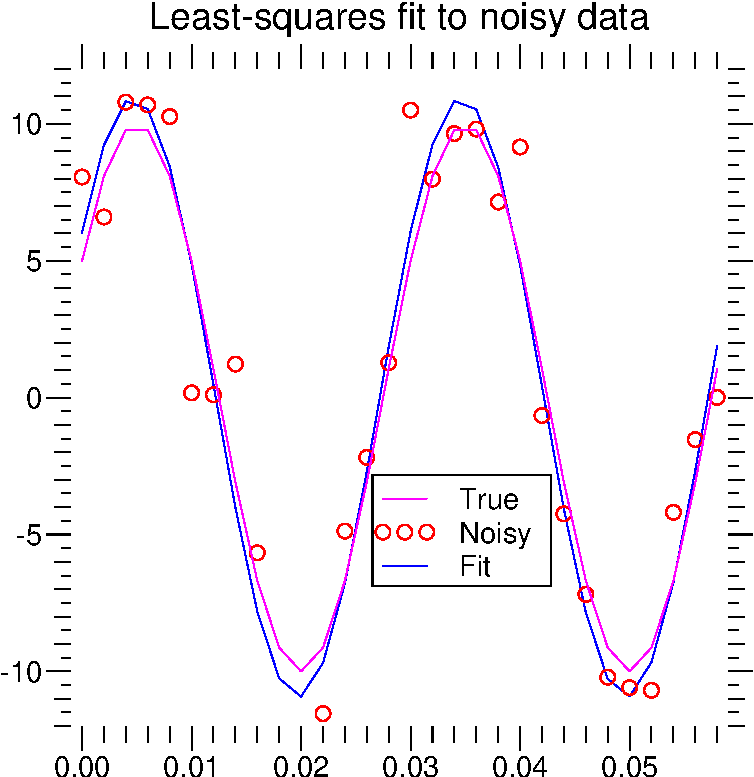
\includegraphics[%
  width=0.50\paperwidth]{leastsqfit.epsi}\end{center}


\caption{\label{fig:least_squares_fit}Least-square fitting to noisy data
using \textbf{scipy.optimize.leastsq}}
\end{figure}



\subsection{Scalar function minimizers}

Often only the minimum of a scalar function is needed (a scalar function
is one that takes a scalar as input and returns a scalar output).
In these circumstances, other optimization techniques have been developed
that can work faster. 


\subsubsection{Unconstrained minimization (optimize.brent)}

There are actually two methods that can be used to minimize a scalar
function (\textbf{brent} and \textbf{golden)}, but \textbf{golden}
is included only for academic purposes and should rarely be used.
The brent method uses Brent's algorithm for locating a minimum. Optimally
a bracket should be given which contains the minimum desired. A bracket
is a triple $\left(a,b,c\right)$ such that $f\left(a\right)>f\left(b\right)<f\left(c\right)$
and $a<b<c$. If this is not given, then alternatively two starting
points can be chosen and a bracket will be found from these points
using a simple marching algorithm. If these two starting points are
not provided 0 and 1 will be used (this may not be the right choice
for your function and result in an unexpected minimum being returned). 


\subsubsection{Bounded minimization (optimize.fminbound)}

Thus far all of the minimization routines described have been unconstrained
minimization routines. Very often, however, there are constraints
that can be placed on the solution space before minimization occurs.
The \textbf{fminbound} function is an example of a constrained minimization
procedure that provides a rudimentary interval constraint for scalar
functions. The interval constraint allows the minimization to occur
only between two fixed endpoints.

For example, to find the minimum of $J_{1}\left(x\right)$ near $x=5$,
\textbf{fminbound} can be called using the interval $\left[4,7\right]$
as a constraint. The result is $x_{\textrm{min}}=5.3314$:

\verbatiminput{example5.8}


\subsection{Root finding }


\subsubsection{Sets of equations}

To find the roots of a polynomial, the command \textbf{roots} is useful.
To find a root of a set of non-linear equations, the command \textbf{optimize.fsolve}
is needed. For example, the following example finds the roots of the
single-variable transcendental equation\[
x+2\cos\left(x\right)=0,\]
 and the set of non-linear equations\begin{eqnarray*}
x_{0}\cos\left(x_{1}\right) & = & 4,\\
x_{0}x_{1}-x_{1} & = & 5.\end{eqnarray*}
 The results are $x=-1.0299$ and $x_{0}=6.5041,\, x_{1}=0.9084$.

\verbatiminput{example5.9}


\subsubsection{Scalar function root finding}

If one has a single-variable equation, there are four different root
finder algorithms that can be tried. Each of these root finding algorithms
requires the endpoints of an interval where a root is suspected (because
the function changes signs). In general \textbf{brentq} is the best
choice, but the other methods may be useful in certain circumstances
or for academic purposes.


\subsubsection{Fixed-point solving}

A problem closely related to finding the zeros of a function is the
problem of finding a fixed-point of a function. A fixed point of a
function is the point at which evaluation of the function returns
the point: $g\left(x\right)=x.$ Clearly the fixed point of $g$ is
the root of $f\left(x\right)=g\left(x\right)-x.$ Equivalently, the
root of $f$ is the fixed\_point of $g\left(x\right)=f\left(x\right)+x.$
The routine \textbf{fixed\_point} provides a simple iterative method
using Aitkens sequence acceleration to estimate the fixed point of
$g$ given a starting point. 


\section{Interpolation (interpolate)}

There are two general interpolation facilities available in SciPy.
The first facility is an interpolation class which performs linear
1-dimensional interpolation. The second facility is based on the FORTRAN
library FITPACK and provides functions for 1- and 2-dimensional (smoothed)
cubic-spline interpolation. 


\subsection{Linear 1-d interpolation (interpolate.linear\_1d)}

The linear\_1d class in scipy.interpolate is a convenient method to
create a function based on fixed data points which can be evaluated
anywhere within the domain defined by the given data using linear
interpolation. An instance of this class is created by passing the
1-d vectors comprising the data. The instance of this class defines
a \emph{\_\_call\_\_} method and can therefore by treated like a function
which interpolates between known data values to obtain unknown values
(it even has a docstring for help). Behavior at the boundary can be
specified at instantiation time. The following example demonstrates
it's use. 

\verbatiminput{example6.1}Figure shows the result: %
\begin{figure}[htbp]
\begin{center}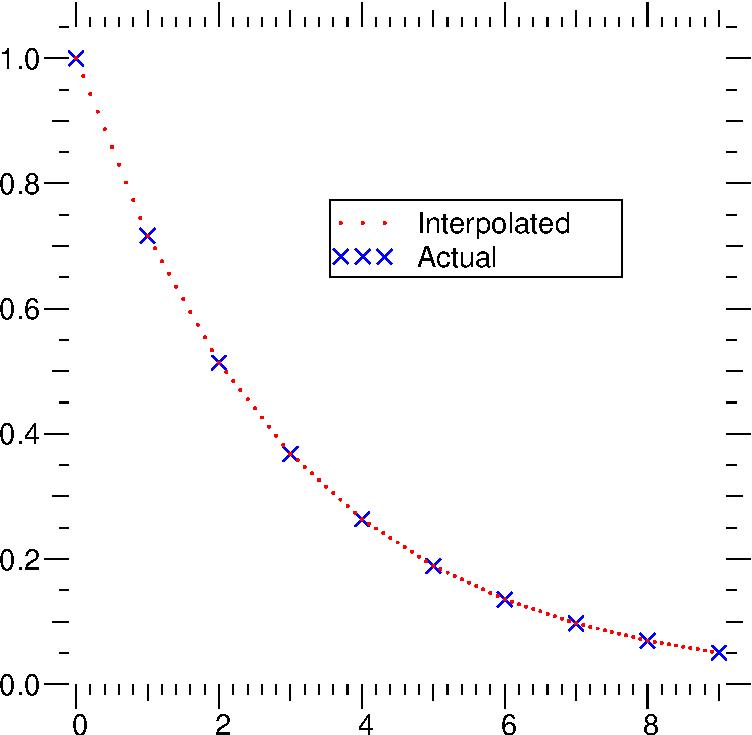
\includegraphics[%
  width=0.50\paperwidth]{inter_1d.epsi}\end{center}


\caption{\label{fig:inter_1d}One-dimensional interpolation using the class
\textbf{interpolate.linear\_1d.}}
\end{figure}



\subsection{Spline interpolation in 1-d (interpolate.splXXX)}

Spline interpolation requires two essential steps: (1) a spline representation
of the curve is computed, and (2) the spline is evaluated at the desired
points. In order to find the spline representation, there are two
different was to represent a curve and obtain (smoothing) spline coefficients:
directly and parametrically. The direct method finds the spline representation
of a curve in a two-dimensional plane using the function \textbf{interpolate.splrep.}
The first two arguments are the only ones required, and these provide
the $x$ and $y$ components of the curve. The normal output is a
3-tuple, $\left(t,c,k\right)$, containing the knot-points, $t$,
the coefficients $c$ and the order $k$ of the spline. The default
spline order is cubic, but this can be changed with the input keyword,
\emph{k.}

For curves in $N$-dimensional space the function \textbf{interpolate.splprep}
allows defining the curve parametrically. For this function only 1
input argument is required. This input is a list of $N$-arrays representing
the curve in $N$-dimensional space. The length of each array is the
number of curve points, and each array provides one component of the
$N$-dimensional data point. The parameter variable is given with
the keword argument, \emph{u,} which defaults to an equally-spaced
monotonic sequence between $0$ and $1$. The default output consists
of two objects: a 3-tuple, $\left(t,c,k\right)$, containing the spline
representation and the parameter variable $u.$ 

The keyword argument, \emph{s}, is used to specify the amount of smoothing
to perform during the spline fit. The default value of $s$ is $s=m-\sqrt{2m}$
where $m$ is the number of data-points being fit. Therefore, \textbf{if
no smoothing is desired a value of $\mathbf{s}=0$ should be passed
to the routines. }

Once the spline representation of the data has been determined, functions
are available for evaluating the spline (\textbf{interpolate.splev)}
and its derivatives (\textbf{interpolate.splev, interpolate.splade})
at any point and the integral of the spline between any two points
(\textbf{interpolate.splint)}. In addition, for cubic splines ($k=3$)
with 8 or more knots, the roots of the spline can be estimated (\textbf{interpolate.sproot)}.
These functions are demonstrated in the example that follows (see
also Figure \ref{fig:spline-1d}).

%
\begin{figure}[htbp]
\begin{center}\subfigure[Cubic-spline (splrep)]{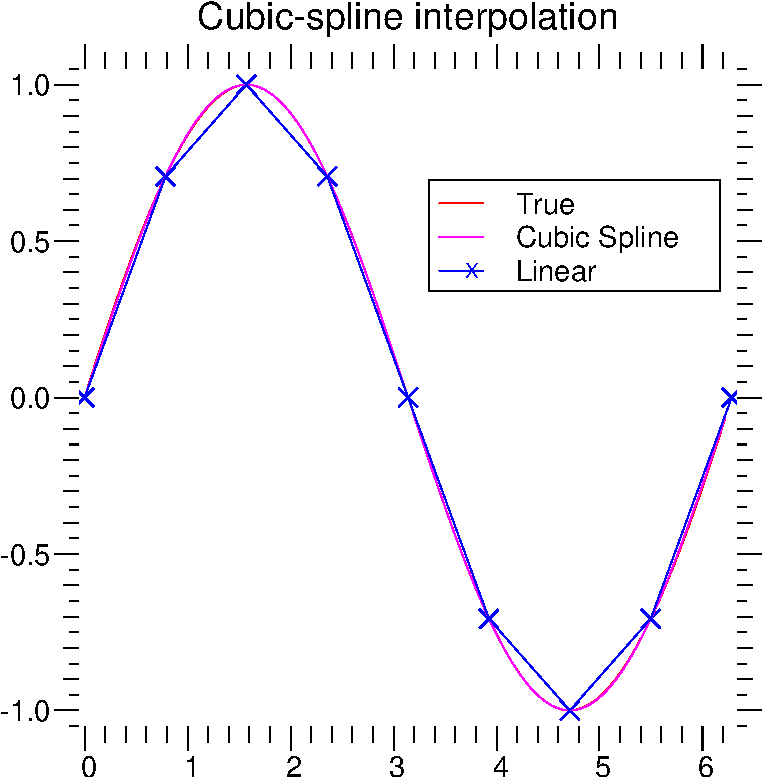
\includegraphics[%
  width=0.40\paperwidth]{interp_cubic.epsi}}\subfigure[Derivative of spline (splev)]{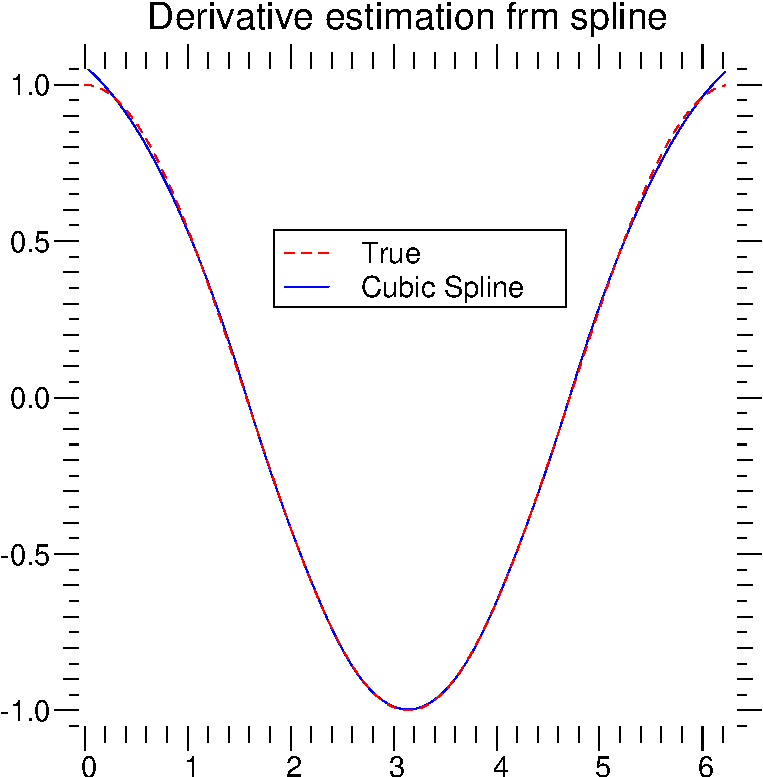
\includegraphics[%
  width=0.40\paperwidth]{interp_cubic_der.epsi}}\end{center}

\begin{center}\subfigure[Integral of spline (splint)]{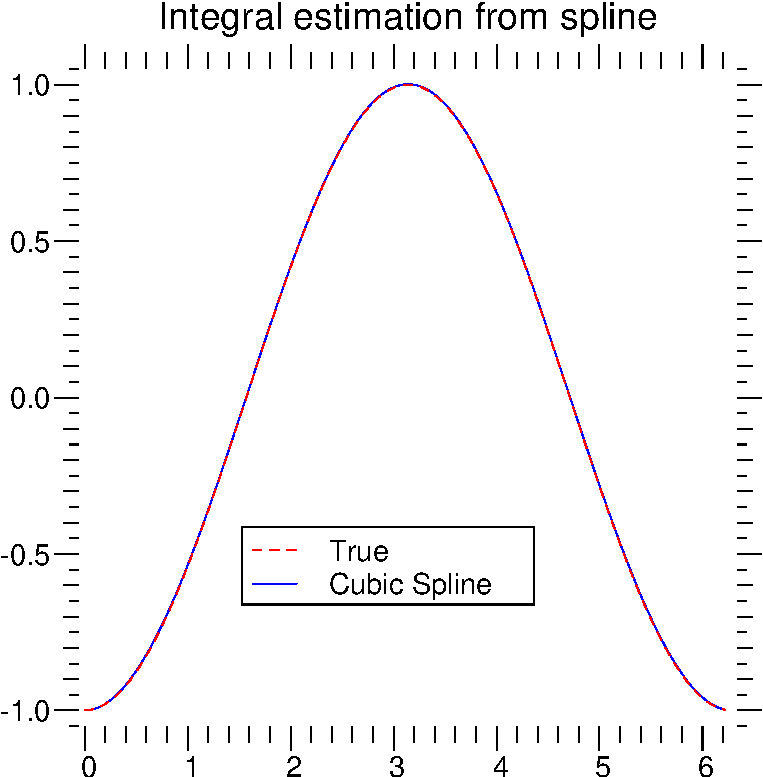
\includegraphics[%
  width=0.40\paperwidth]{interp_cubic_int.epsi}}\subfigure[Spline of parametric curve (splprep)]{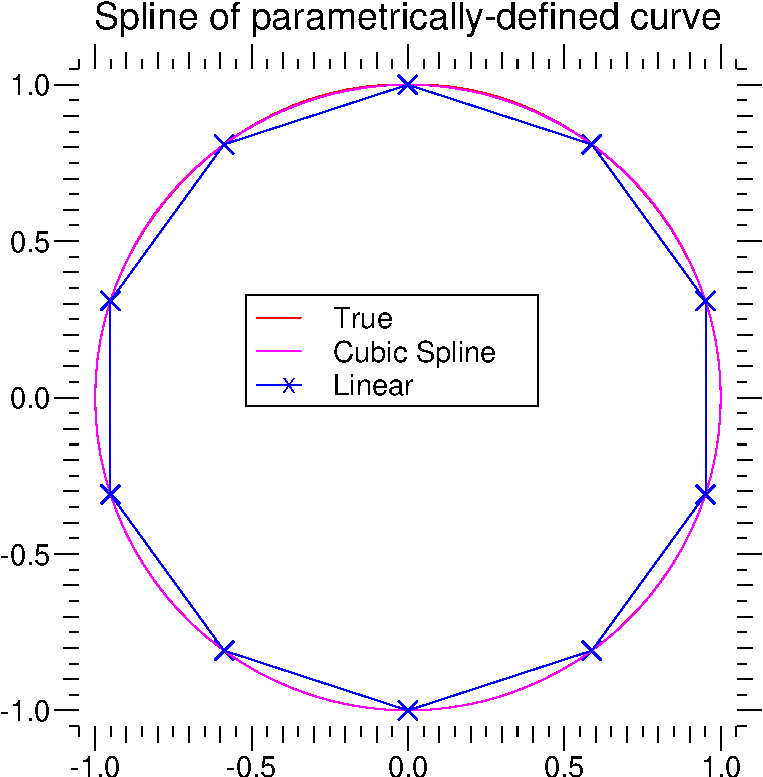
\includegraphics[%
  width=0.40\paperwidth]{interp_cubic_param.epsi}}\end{center}


\caption{\label{fig:spline-1d}Examples of using cubic-spline interpolation.}
\end{figure}


\verbatiminput{example6.2}


\subsection{Two-dimensionsal spline representation (interpolate.bisplrep)}

For (smooth) spline-fitting to a two dimensional surface, the function
\textbf{interpolate.bisplrep} is available. This function takes as
required inputs the \textbf{1-D} arrays \emph{x, y,} and \emph{z}
which represent points on the surface $z=f\left(x,y\right).$ The
default output is a list $\left[tx,ty,c,kx,ky\right]$ whose entries
represent respectively, the components of the knot positions, the
coefficients of the spline, and the order of the spline in each coordinate.
It is convenient to hold this list in a single object, \emph{tck,}
so that it can be passed easily to the function \textbf{interpolate.bisplev.}
The keyword, \emph{s}, \emph{}can be used to change the amount of
smoothing performed on the data while determining the appropriate
spline. The default value is $s=m-\sqrt{2m}$ where $m$ is the number
of data points in the \emph{x, y,} and \emph{z} vectors. As a result,
if no smoothing is desired, then $s=0$ should be passed to \textbf{interpolate.bisplrep.}

To evaluate the two-dimensional spline and it's partial derivatives
(up to the order of the spline), the function \textbf{interpolate.bisplev}
is required. This function takes as the first two arguments \textbf{two
1-D arrays} whose cross-product specifies the domain over which to
evaluate the spline. The third argument is the \emph{tck} list returned
from \textbf{interpolate.bisplrep.} If desired, the fourth and fifth
arguments provide the orders of the partial derivative in the $x$
and $y$ direction respectively. 

It is important to note that two dimensional interpolation should
not be used to find the spline representation of images. The algorithm
used is not amenable to large numbers of input points. The signal
processing toolbox contains (soon) more appropriate algorithms for
finding the spline representation of an image. The two dimensional
interpolation commands are intended for use when interpolating a two
dimensional function as shown in the example that follows (See also
Figure \ref{fig:2d_interp}). This example uses the \textbf{mgrid}
command in SciPy which is useful for defining a {}``mesh-grid''
in many dimensions. (See also the \textbf{ogrid} command if the full-mesh
is not needed). The number of output arguments and the number of dimensions
of each argument is determined by the number of indexing objects passed
in \textbf{mgrid{[}{]}.} \verbatiminput{example6.3}

\vspace{0.3cm}
\begin{center}%
\begin{figure}[htbp]
\begin{center}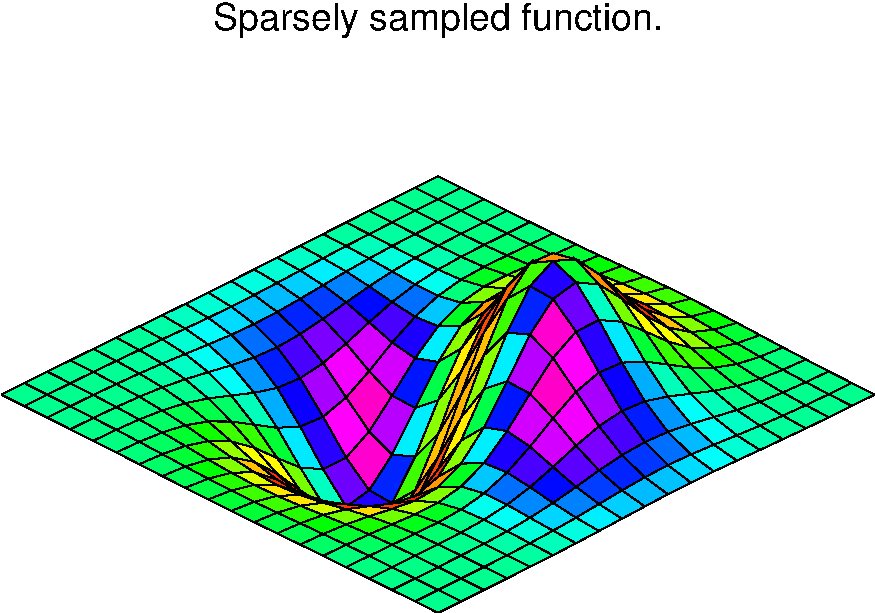
\includegraphics[%
  width=0.40\paperwidth]{2d_func.epsi}~~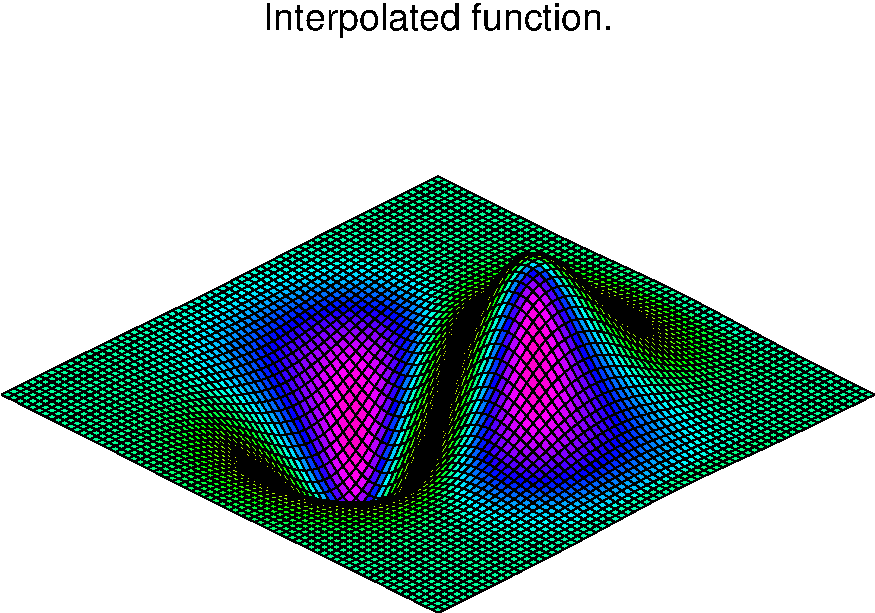
\includegraphics[%
  width=0.45\paperwidth]{2d_interp.epsi}\end{center}


\caption{\label{fig:2d_interp}Example of two-dimensional spline interpolation.}
\end{figure}
\end{center}
\vspace{0.3cm}


\section{Signal Processing (signal)}

The signal processing toolbox currently contains some filtering functions,
a limited set of filter design tools, and a few B-spline interpolation
algorithms for one- and two-dimensional data. While the B-spline algorithms
could technically be placed under the interpolation category, they
are included here because they only work with equally-spaced data
and make heavy use of filter-theory and transfer-function formalism
to provide a fast B-spline transform. To understand this section you
will need to understand that a signal in SciPy is an array of real
or complex numbers. 


\subsection{B-splines}

A B-spline is an approximation of a continuous function over a finite-domain
in terms of B-spline coefficients and knot points. If the knot-points
are equally spaced with spacing $\Delta x$, then the B-spline approximation
to a 1-dimensional function is the finite-basis expansion. \[
y\left(x\right)\approx\sum_{j}c_{j}\beta^{o}\left(\frac{x}{\Delta x}-j\right).\]
 In two dimensions with knot-spacing $\Delta x$ and $\Delta y$,
the function representation is \[
z\left(x,y\right)\approx\sum_{j}\sum_{k}c_{jk}\beta^{o}\left(\frac{x}{\Delta x}-j\right)\beta^{o}\left(\frac{y}{\Delta y}-k\right).\]
 In these expressions, $\beta^{o}\left(\cdot\right)$ is the space-limited
B-spline basis function of order, $o$. The requirement of equally-spaced
knot-points and equally-spaced data points, allows the development
of fast (inverse-filtering) algorithms for determining the coefficients,
$c_{j}$, from sample-values, $y_{n}$. Unlike the general spline
interpolation algorithms, these algorithms can quickly find the spline
coefficients for large images. 

The advantage of representing a set of samples via B-spline basis
functions is that continuous-domain operators (derivatives, re-sampling,
integral, etc.) which assume that the data samples are drawn from
an underlying continuous function can be computed with relative ease
from the spline coefficients. For example, the second-derivative of
a spline is \[
y\prime^{\prime\prime}\left(x\right)=\frac{1}{\Delta x^{2}}\sum_{j}c_{j}\beta^{o\prime\prime}\left(\frac{x}{\Delta x}-j\right).\]
 Using the property of B-splines that \[
\frac{d^{2}\beta^{o}\left(w\right)}{dw^{2}}=\beta^{o-2}\left(w+1\right)-2\beta^{o-2}\left(w\right)+\beta^{o-2}\left(w-1\right)\]
 it can be seen that \[
y^{\prime\prime}\left(x\right)=\frac{1}{\Delta x^{2}}\sum_{j}c_{j}\left[\beta^{o-2}\left(\frac{x}{\Delta x}-j+1\right)-2\beta^{o-2}\left(\frac{x}{\Delta x}-j\right)+\beta^{o-2}\left(\frac{x}{\Delta x}-j-1\right)\right].\]
 If $o=3$, then at the sample points, \begin{eqnarray*}
\Delta x^{2}\left.y^{\prime}\left(x\right)\right|_{x=n\Delta x} & = & \sum_{j}c_{j}\delta_{n-j+1}-2c_{j}\delta_{n-j}+c_{j}\delta_{n-j-1},\\
 & = & c_{n+1}-2c_{n}+c_{n-1}.\end{eqnarray*}
 Thus, the second-derivative signal can be easily calculated from
the spline fit. if desired, smoothing splines can be found to make
the second-derivative less sensitive to random-errors. 

The savvy reader will have already noticed that the data samples are
related to the knot coefficients via a convolution operator, so that
simple convolution with the sampled B-spline function recovers the
original data from the spline coefficients. The output of convolutions
can change depending on how boundaries are handled (this becomes increasingly
more important as the number of dimensions in the data-set increases).
The algorithms relating to B-splines in the signal-processing sub
package assume mirror-symmetric boundary conditions. Thus, spline
coefficients are computed based on that assumption, and data-samples
can be recovered exactly from the spline coefficients by assuming
them to be mirror-symmetric also.

Currently the package provides functions for determining seond- and
third-order cubic spline coefficients from equally spaced samples
in one- and two-dimensions (\textbf{signal.qspline1d, signal.qspline2d,
signal.cspline1d, signal.cspline2d}). The package also supplies a
function (\textbf{signal.bspline}) for evaluating the bspline basis
function, $\beta^{o}\left(x\right)$ for arbitrary order and $x.$
For large $o$, the B-spline basis function can be approximated well
by a zero-mean Gaussian function with standard-deviation equal to
$\sigma_{o}=\left(o+1\right)/12$:\[
\beta^{o}\left(x\right)\approx\frac{1}{\sqrt{2\pi\sigma_{o}^{2}}}\exp\left(-\frac{x^{2}}{2\sigma_{o}}\right).\]
 A function to compute this Gaussian for arbitrary $x$ and $o$ is
also available (\textbf{signal.gauss\_spline}). The following code
and Figure uses spline-filtering to compute an edge-image (the second-derivative
of a smoothed spline) of Lena's face which is an array returned by
the command \textbf{lena().} The command \textbf{signal.sepfir2d}
was used to apply a separable two-dimensional FIR filter with mirror-symmetric
boundary conditions to the spline coefficients. This function is ideally
suited for reconstructing samples from spline coefficients and is
faster than \textbf{signal.convolve2d} which convolves arbitrary two-dimensional
filters and allows for choosing mirror-symmetric boundary conditions. 

\verbatiminput{example6.4}

%
\begin{figure}[htbp]
\begin{center}\includegraphics[%
  width=0.40\paperwidth]{lena_image.epsi}~~\includegraphics[%
  width=0.40\paperwidth]{lena_edge.epsi}\end{center}


\caption{\label{fig:lena_edge_spline}Example of using smoothing splines to
filter images.}
\end{figure}



\subsection{Filtering}

Filtering is a generic name for any system that modifies an input
signal in some way. In SciPy a signal can be thought of as a Numeric
array. There are different kinds of filters for different kinds of
operations. There are two broad kinds of filtering operations: linear
and non-linear. Linear filters can always be reduced to multiplication
of the flattened Numeric array by an appropriate matrix resulting
in another flattened Numeric array. Of course, this is not usually
the best way to compute the filter as the matrices and vectors involved
may be huge. For example filtering a $512\times512$ image with this
method would require multiplication of a $512^{2}x512^{2}$matrix
with a $512^{2}$ vector. Just trying to store the $512^{2}\times512^{2}$
matrix using a standard Numeric array would require $68,719,476,736$
elements. At 4 bytes per element this would require $256\textrm{GB}$
of memory. In most applications most of the elements of this matrix
are zero and a different method for computing the output of the filter
is employed.


\subsubsection{Convolution/Correlation}

Many linear filters also have the property of shift-invariance. This
means that the filtering operation is the same at different locations
in the signal and it implies that the filtering matrix can be constructed
from knowledge of one row (or column) of the matrix alone. In this
case, the matrix multiplication can be accomplished using Fourier
transforms.

Let $x\left[n\right]$ define a one-dimensional signal indexed by
the integer $n.$ Full convolution of two one-dimensional signals
can be expressed as \[
y\left[n\right]=\sum_{k=-\infty}^{\infty}x\left[k\right]h\left[n-k\right].\]
 This equation can only be implemented directly if we limit the sequences
to finite support sequences that can be stored in a computer, choose
$n=0$ to be the starting point of both sequences, let $K+1$ be that
value for which $y\left[n\right]=0$ for all $n>K+1$ and $M+1$ be
that value for which $x\left[n\right]=0$ for all $n>M+1$, then the
discrete convolution expression is \[
y\left[n\right]=\sum_{k=\max\left(n-M,0\right)}^{\min\left(n,K\right)}x\left[k\right]h\left[n-k\right].\]
 For convenience assume $K\geq M.$ Then, more explicitly the output
of this operation is \begin{eqnarray*}
y\left[0\right] & = & x\left[0\right]h\left[0\right]\\
y\left[1\right] & = & x\left[0\right]h\left[1\right]+x\left[1\right]h\left[0\right]\\
y\left[2\right] & = & x\left[0\right]h\left[2\right]+x\left[1\right]h\left[1\right]+x\left[2\right]h\left[0\right]\\
\vdots & \vdots & \vdots\\
y\left[M\right] & = & x\left[0\right]h\left[M\right]+x\left[1\right]h\left[M-1\right]+\cdots+x\left[M\right]h\left[0\right]\\
y\left[M+1\right] & = & x\left[1\right]h\left[M\right]+x\left[2\right]h\left[M-1\right]+\cdots+x\left[M+1\right]h\left[0\right]\\
\vdots & \vdots & \vdots\\
y\left[K\right] & = & x\left[K-M\right]h\left[M\right]+\cdots+x\left[K\right]h\left[0\right]\\
y\left[K+1\right] & = & x\left[K+1-M\right]h\left[M\right]+\cdots+x\left[K\right]h\left[1\right]\\
\vdots & \vdots & \vdots\\
y\left[K+M-1\right] & = & x\left[K-1\right]h\left[M\right]+x\left[K\right]h\left[M-1\right]\\
y\left[K+M\right] & = & x\left[K\right]h\left[M\right].\end{eqnarray*}
 Thus, the full discrete convolution of two finite sequences of lengths
$K+1$ and $M+1$ respectively results in a finite sequence of length
$K+M+1=\left(K+1\right)+\left(M+1\right)-1.$ 

One dimensional convolution is implemented in SciPy with the function
\texttt{signal.convolve}. This function takes as inputs the signals
$x,$ $h$, and an optional flag and returns the signal $y.$ The
optional flag allows for specification of which part of the output
signal to return. The default value of 'full' returns the entire signal.
If the flag has a value of 'same' then only the middle $K$ values
are returned starting at $y\left[\left\lfloor \frac{M-1}{2}\right\rfloor \right]$
so that the output has the same length as the largest input. If the
flag has a value of 'valid' then only the middle $K-M+1=\left(K+1\right)-\left(M+1\right)+1$
output values are returned where $z$ depends on all of the values
of the smallest input from $h\left[0\right]$ to $h\left[M\right].$
In other words only the values $y\left[M\right]$ to $y\left[K\right]$
inclusive are returned.

This same function \texttt{signal.convolve} can actually take $N$-dimensional
arrays as inputs and will return the $N$-dimensional convolution
of the two arrays. The same input flags are available for that case
as well. 

Correlation is very similar to convolution except for the minus sign
becomes a plus sign. Thus \[
w\left[n\right]=\sum_{k=-\infty}^{\infty}y\left[k\right]x\left[n+k\right]\]
 is the (cross) correlation of the signals $y$ and $x.$ For finite-length
signals with $y\left[n\right]=0$ outside of the range $\left[0,K\right]$
and $x\left[n\right]=0$ outside of the range $\left[0,M\right],$
the summation can simplify to \[
w\left[n\right]=\sum_{k=\max\left(0,-n\right)}^{\min\left(K,M-n\right)}y\left[k\right]x\left[n+k\right].\]
Assuming again that $K\geq M$ this is \begin{eqnarray*}
w\left[-K\right] & = & y\left[K\right]x\left[0\right]\\
w\left[-K+1\right] & = & y\left[K-1\right]x\left[0\right]+y\left[K\right]x\left[1\right]\\
\vdots & \vdots & \vdots\\
w\left[M-K\right] & = & y\left[K-M\right]x\left[0\right]+y\left[K-M+1\right]x\left[1\right]+\cdots+y\left[K\right]x\left[M\right]\\
w\left[M-K+1\right] & = & y\left[K-M-1\right]x\left[0\right]+\cdots+y\left[K-1\right]x\left[M\right]\\
\vdots & \vdots & \vdots\\
w\left[-1\right] & = & y\left[1\right]x\left[0\right]+y\left[2\right]x\left[1\right]+\cdots+y\left[M+1\right]x\left[M\right]\\
w\left[0\right] & = & y\left[0\right]x\left[0\right]+y\left[1\right]x\left[1\right]+\cdots+y\left[M\right]x\left[M\right]\\
w\left[1\right] & = & y\left[0\right]x\left[1\right]+y\left[1\right]x\left[2\right]+\cdots+y\left[M-1\right]x\left[M\right]\\
w\left[2\right] & = & y\left[0\right]x\left[2\right]+y\left[1\right]x\left[3\right]+\cdots+y\left[M-2\right]x\left[M\right]\\
\vdots & \vdots & \vdots\\
w\left[M-1\right] & = & y\left[0\right]x\left[M-1\right]+y\left[1\right]x\left[M\right]\\
w\left[M\right] & = & y\left[0\right]x\left[M\right].\end{eqnarray*}


The SciPy function \texttt{signal.correlate} implements this operation.
Equivalent flags are available for this operation to return the full
$K+M+1$ length sequence ('full') or a sequence with the same size
as the largest sequence starting at $w\left[-K+\left\lfloor \frac{M-1}{2}\right\rfloor \right]$
('same') or a sequence where the values depend on all the values of
the smallest sequence ('valid'). This final option returns the $K-M+1$
values $w\left[M-K\right]$ to $w\left[0\right]$ inclusive. 

The function \textbf{signal.correlate} can also take arbitrary $N$-dimensional
arrays as input and return the $N$-dimensional convolution of the
two arrays on output. 

When $N=2,$ \textbf{signal.correlate} and/or \textbf{signal.convolve}
can be used to construct arbitrary image filters to perform actions
such as blurring, enhancing, and edge-detection for an image. 

Convolution is mainly used for filtering when one of the signals is
much smaller than the other ($K\gg M$), otherwise linear filtering
is more easily accomplished in the frequency domain (see Fourier Transforms). 


\subsubsection{Difference-equation filtering}

A general class of linear one-dimensional filters (that includes convolution
filters) are filters described by the difference equation \[
\sum_{k=0}^{N}a_{k}y\left[n-k\right]=\sum_{k=0}^{M}b_{k}x\left[n-k\right]\]
 where $x\left[n\right]$ is the input sequence and $y\left[n\right]$
is the output sequence. If we assume initial rest so that $y\left[n\right]=0$
for $n<0$, then this kind of filter can be implemented using convolution.
However, the convolution filter sequence $h\left[n\right]$ could
be infinite if $a_{k}\neq0$ for $k\geq1.$ In addition, this general
class of linear filter allows initial conditions to be placed on $y\left[n\right]$
for $n<0$ resulting in a filter that cannot be expressed using convolution.

The difference equation filter can be thought of as finding $y\left[n\right]$
recursively in terms of it's previous values \[
a_{0}y\left[n\right]=-a_{1}y\left[n-1\right]-\cdots-a_{N}y\left[n-N\right]+\cdots+b_{0}x\left[n\right]+\cdots+b_{M}x\left[n-M\right].\]
Often $a_{0}=1$ is chosen for normalization. The implementation in
SciPy of this general difference equation filter is a little more
complicated then would be implied by the previous equation. It is
implemented so that only one signal needs to be delayed. The actual
implementation equations are (assuming $a_{0}=1$). \begin{eqnarray*}
y\left[n\right] & = & b_{0}x\left[n\right]+z_{0}\left[n-1\right]\\
z_{0}\left[n\right] & = & b_{1}x\left[n\right]+z_{1}\left[n-1\right]-a_{1}y\left[n\right]\\
z_{1}\left[n\right] & = & b_{2}x\left[n\right]+z_{2}\left[n-1\right]-a_{2}y\left[n\right]\\
\vdots & \vdots & \vdots\\
z_{K-2}\left[n\right] & = & b_{K-1}x\left[n\right]+z_{K-1}\left[n-1\right]-a_{K-1}y\left[n\right]\\
z_{K-1}\left[n\right] & = & b_{K}x\left[n\right]-a_{K}y\left[n\right],\end{eqnarray*}
where $K=\max\left(N,M\right).$ Note that $b_{K}=0$ if $K>M$ and
$a_{K}=0$ if $K>N.$ In this way, the output at time $n$ depends
only on the input at time $n$ and the value of $z_{0}$ at the previous
time. This can always be calculated as long as the $K$ values $z_{0}\left[n-1\right]\ldots z_{K-1}\left[n-1\right]$
are computed and stored at each time step. 

The difference-equation filter is called using the command \textbf{signal.lfilter}
in SciPy. This command takes as inputs the vector $b,$ the vector,
$a,$ a signal $x$ and returns the vector $y$ (the same length as
$x$) computed using the equation given above. If $x$ is $N$-dimensional,
then the filter is computed along the axis provided. If, desired,
initial conditions providing the values of $z_{0}\left[-1\right]$
to $z_{K-1}\left[-1\right]$ can be provided or else it will be assumed
that they are all zero. If initial conditions are provided, then the
final conditions on the intermediate variables are also returned.
These could be used, for example, to restart the calculation in the
same state.

Sometimes it is more convenient to express the initial conditions
in terms of the signals $x\left[n\right]$ and $y\left[n\right].$
In other words, perhaps you have the values of $x\left[-M\right]$
to $x\left[-1\right]$ and the values of $y\left[-N\right]$ to $y\left[-1\right]$
and would like to determine what values of $z_{m}\left[-1\right]$
should be delivered as initial conditions to the difference-equation
filter. It is not difficult to show that for $0\leq m<K,$\[
z_{m}\left[n\right]=\sum_{p=0}^{K-m-1}\left(b_{m+p+1}x\left[n-p\right]-a_{m+p+1}y\left[n-p\right]\right).\]
 Using this formula we can find the intial condition vector $z_{0}\left[-1\right]$
to $z_{K-1}\left[-1\right]$ given initial conditions on $y$ (and
$x$). The command \textbf{signal.lfiltic} performs this function.


\subsubsection{Other filters}

The signal processing package affords many more filters as well. 


\paragraph{Median Filter}

A median filter is commonly applied when noise is markedly non-Gaussian
or when it is desired to preserve edges. The median filter works by
sorting all of the array pixel values in a rectangular region surrounding
the point of interest. The sample median of this list of neighborhood
pixel values is used as the value for the output array. The sample
median is the middle array value in a sorted list of neighborhood
values. If there are an even number of elements in the neighborhood,
then the average of the middle two values is used as the median. A
general purpose median filter that works on N-dimensional arrays is
\textbf{signal.medfilt}. A specialized version that works only for
two-dimensional arrays is available as \textbf{signal.medfilt2d}. \texttt{}


\paragraph{Order Filter}

A median filter is a specific example of a more general class of filters
called order filters. To compute the output at a particular pixel,
all order filters use the array values in a region surrounding that
pixel. These array values are sorted and then one of them is selected
as the output value. For the median filter, the sample median of the
list of array values is used as the output. A general order filter
allows the user to select which of the sorted values will be used
as the output. So, for example one could choose to pick the maximum
in the list or the minimum. The order filter takes an additional argument
besides the input array and the region mask that specifies which of
the elements in the sorted list of neighbor array values should be
used as the output. The command to perform an order filter is \textbf{signal.order\_filter}. 


\paragraph{Wiener filter}

The Wiener filter is a simple deblurring filter for denoising images.
This is not the Wiener filter commonly described in image reconstruction
problems but instead it is a simple, local-mean filter. Let $x$ be
the input signal, then the output is

\[
y=\left\{ \begin{array}{cc}
\frac{\sigma^{2}}{\sigma_{x}^{2}}m_{x}+\left(1-\frac{\sigma^{2}}{\sigma_{x}^{2}}\right)x & \sigma_{x}^{2}\geq\sigma^{2},\\
m_{x} & \sigma_{x}^{2}<\sigma^{2}.\end{array}\right.\]
 Where $m_{x}$ is the local estimate of the mean and $\sigma_{x}^{2}$
is the local estimate of the variance. The window for these estimates
is an optional input parameter (default is $3\times3$). The parameter
$\sigma^{2}$ is a threshold noise parameter. If $\sigma$ is not
given then it is estimated as the average of the local variances. 


\paragraph{Hilbert filter}

The Hilbert transform constructs the complex-valued analytic signal
from a real signal. For example if $x=\cos\omega n$ then $y=\textrm{hilbert}\left(x\right)$
would return (except near the edges) $y=\exp\left(j\omega n\right).$
In the frequency domain, the hilbert transform performs\[
Y=X\cdot H\]
 where $H$ is 2 for positive frequencies, $0$ for negative frequencies
and $1$ for zero-frequencies. 


\paragraph{Detrend}


\subsection{Filter design}


\subsubsection{Finite-impulse response design }


\subsubsection{Inifinite-impulse response design}


\subsubsection{Analog filter frequency response}


\subsubsection{Digital filter frequency response}


\subsection{Linear Time-Invariant Systems}


\subsubsection{LTI Object}


\subsubsection{Continuous-Time Simulation}


\subsubsection{Step response}


\subsubsection{Impulse response}


\section{Input/Output}


\subsection{Binary }


\subsubsection{Arbitrary binary input and output (fopen)}


\subsubsection{Read and write Matlab .mat files}


\subsubsection{Saving workspace}


\subsection{Text-file }


\subsubsection{Read text-files (read\_array)}


\subsubsection{Write a text-file (write\_array)}


\section{Fourier Transforms}


\subsection{One-dimensional}


\subsection{Two-dimensional}


\subsection{N-dimensional}


\subsection{Shifting}


\subsection{Sample frequencies}


\subsection{Hilbert transform}


\subsection{Tilbert transform}


\section{Linear Algebra}

When SciPy is built using the optimized ATLAS LAPACK and BLAS libraries,
it has very fast linear algebra capabilities. If you dig deep enough,
all of the raw lapack and blas libraries are available for your use
for even more speed. In this section, some easier-to-use interfaces
to these routines are described.

All of these linear algebra routines expect an object that can be
converted into a 2-dimensional array. The output of these routines
is also a two-dimensional array. There is a matrix class defined in
Numeric that scipy inherits and extends. You can initialize this class
with an appropriate Numeric array in order to get objects for which
multiplication is matrix-multiplication instead of the default, element-by-element
multiplication. 


\subsection{Matrix Class}

The matrix class is initialized with the SciPy command \texttt{\textbf{mat}}
which is just convenient short-hand for \texttt{\textbf{Matrix.Matrix}}.
If you are going to be doing a lot of matrix-math, it is convenient
to convert arrays into matrices using this command. One convencience
of using the mat command is that you can enter two-dimensional matrices
in using MATLAB-like syntax with commas or spaces separating columns
and semicolons separting rows as long as the matrix is placed in a
string passed to \textbf{mat}. 


\subsection{Basic routines}


\subsubsection{Finding Inverse}

The inverse of a matrix $\mathbf{A}$ is the matrix $\mathbf{B}$
such that $\mathbf{AB}=\mathbf{I}$ where $\mathbf{I}$ is the identity
matrix consisting of ones down the main diagonal. Usually $\mathbf{B}$
is denoted $\mathbf{B}=\mathbf{A}^{-1}$. In SciPy, the matrix inverse
of the Numeric array, A, is obtained using \texttt{\textbf{linalg.inv}}\texttt{(A)},
or using \texttt{A.I} if \texttt{A} is a Matrix. For example, let
\[
\mathbf{A=}\left[\begin{array}{ccc}
1 & 3 & 5\\
2 & 5 & 1\\
2 & 3 & 8\end{array}\right]\]
then \[
\mathbf{A^{-1}=\frac{1}{25}\left[\begin{array}{ccc}
-37 & 9 & 22\\
14 & 2 & -9\\
4 & -3 & 1\end{array}\right]=\left[\begin{array}{ccc}
-1.48 & 0.36 & 0.88\\
0.56 & 0.08 & -0.36\\
0.16 & -0.12 & 0.04\end{array}\right].}\]
 The following example demonstrates this computation in SciPy\verbatiminput{example10.2.1}


\subsubsection{Solving linear system}

Solving linear systems of equations is straightforward using the scipy
command \textbf{linalg.solve.} This command expects an input matrix
and a right-hand-side vector. The solution vector is then computed.
An option for entering a symmetrix matrix is offered which can speed
up the processing when applicable. As an example, suppose it is desired
to solve the following simultaneous equations: \begin{eqnarray*}
x+3y+5z & = & 10\\
2x+5y+z & = & 8\\
2x+3y+8z & = & 3\end{eqnarray*}
 We could find the solution vector using a matrix inverse: \[
\left[\begin{array}{c}
x\\
y\\
z\end{array}\right]=\left[\begin{array}{ccc}
1 & 3 & 5\\
2 & 5 & 1\\
2 & 3 & 8\end{array}\right]^{-1}\left[\begin{array}{c}
10\\
8\\
3\end{array}\right]=\frac{1}{25}\left[\begin{array}{c}
-232\\
129\\
19\end{array}\right]=\left[\begin{array}{c}
-9.28\\
5.16\\
0.76\end{array}\right].\]
 However, it is better to use the linalg.solve command which can be
faster and more numerically stable. In this case it gives the same
answer as shown in the following example: \verbatiminput{example10.2.2}


\subsubsection{Finding Determinant}

The determinant of a square matrix $\mathbf{A}$ is often denoted
$\left|\mathbf{A}\right|$ and is a quantity often used in linear
algebra. Suppose $a_{ij}$ are the elements of the matrix $\mathbf{A}$
and let $M_{ij}=\left|\mathbf{A}_{ij}\right|$ be the determinant
of the matrix left by removing the $i^{\textrm{th}}$ row and $j^{\textrm{th}}$column
from $\mathbf{A}$. Then for any row $i,$\[
\left|\mathbf{A}\right|=\sum_{j}\left(-1\right)^{i+j}a_{ij}M_{ij}.\]
 This is a recursive way to define the determinant where the base
case is defined by accepting that the determinant of a $1\times1$
matrix is the only matrix element. In SciPy the determinant can be
calculated with \textbf{linalg.det}. For example, the determinant
of \[
\mathbf{A=}\left[\begin{array}{ccc}
1 & 3 & 5\\
2 & 5 & 1\\
2 & 3 & 8\end{array}\right]\]
is \begin{eqnarray*}
\left|\mathbf{A}\right| & = & 1\left|\begin{array}{cc}
5 & 1\\
3 & 8\end{array}\right|-3\left|\begin{array}{cc}
2 & 1\\
2 & 8\end{array}\right|+5\left|\begin{array}{cc}
2 & 5\\
2 & 3\end{array}\right|\\
 & = & 1\left(5\cdot8-3\cdot1\right)-3\left(2\cdot8-2\cdot1\right)+5\left(2\cdot3-2\cdot5\right)=-25.\end{eqnarray*}
 In SciPy this is computed as shown in this example:

\verbatiminput{example10.2.3}


\subsubsection{Computing norms}

Matrix and vector norms can also be computed with SciPy. A wide range
of norm definitions are available using different parameters to the
order argument of \textbf{linalg.norm}. This function takes a rank-1
(vectors) or a rank-2 (matrices) array and an optional order argument
(default is 2). Based on these inputs a vector or matrix norm of the
requested order is computed. 

For vector \textbf{x}, the order parameter can be any real number
including \textbf{inf} or -\textbf{inf}. The computed norm is \[
\left\Vert \mathbf{x}\right\Vert =\left\{ \begin{array}{cc}
\max\left|x_{i}\right| & \textrm{ord}=\textrm{inf}\\
\min\left|x_{i}\right| & \textrm{ord}=-\textrm{inf}\\
\left(\sum_{i}\left|x_{i}\right|^{\textrm{ord}}\right)^{1/\textrm{ord}} & \left|\textrm{ord}\right|<\infty.\end{array}\right.\]


For matrix $\mathbf{A}$ the only valid values for norm are $\pm2,\pm1,$
$\pm$inf, and 'fro' (or 'f') Thus, \[
\left\Vert \mathbf{A}\right\Vert =\left\{ \begin{array}{cc}
\max_{i}\sum_{j}\left|a_{ij}\right| & \textrm{ord}=\textrm{inf}\\
\min_{i}\sum_{j}\left|a_{ij}\right| & \textrm{ord}=-\textrm{inf}\\
\max_{j}\sum_{i}\left|a_{ij}\right| & \textrm{ord}=1\\
\min_{j}\sum_{i}\left|a_{ij}\right| & \textrm{ord}=-1\\
\max\sigma_{i} & \textrm{ord}=2\\
\min\sigma_{i} & \textrm{ord}=-2\\
\sqrt{\textrm{trace}\left(\mathbf{A}^{H}\mathbf{A}\right)} & \textrm{ord}=\textrm{'fro'}\end{array}\right.\]
 where $\sigma_{i}$ are the singular values of $\mathbf{A}$. 


\subsubsection{Solving linear least-squares problems and pseudo-inverses}

Linear least-squares problems occur in many branches of applied mathematics.
In this problem a set of linear scaling coefficients is sought that
allow a model to fit data. In particular it is assumed that data $y_{i}$
is related to data $\mathbf{x}_{i}$ through a set of coefficients
$c_{j}$ and model functions $f_{j}\left(\mathbf{x}_{i}\right)$ via
the model \[
y_{i}=\sum_{j}c_{j}f_{j}\left(\mathbf{x}_{i}\right)+\epsilon_{i}\]
 where $\epsilon_{i}$ represents uncertainty in the data. The strategy
of least squares is to pick the coefficients $c_{j}$ to minimize
\[
J\left(\mathbf{c}\right)=\sum_{i}\left|y_{i}-\sum_{j}c_{j}f_{j}\left(x_{i}\right)\right|^{2}.\]
 

Theoretically, a global minimum will occur when \[
\frac{\partial J}{\partial c_{n}^{*}}=0=\sum_{i}\left(y_{i}-\sum_{j}c_{j}f_{j}\left(x_{i}\right)\right)\left(-f_{n}^{*}\left(x_{i}\right)\right)\]
or \begin{eqnarray*}
\sum_{j}c_{j}\sum_{i}f_{j}\left(x_{i}\right)f_{n}^{*}\left(x_{i}\right) & = & \sum_{i}y_{i}f_{n}^{*}\left(x_{i}\right)\\
\mathbf{A}^{H}\mathbf{Ac} & = & \mathbf{A}^{H}\mathbf{y}\end{eqnarray*}
 where \[
\left\{ \mathbf{A}\right\} _{ij}=f_{j}\left(x_{i}\right).\]
 When $\mathbf{A^{H}A}$ is invertible, then \[
\mathbf{c}=\left(\mathbf{A}^{H}\mathbf{A}\right)^{-1}\mathbf{A}^{H}\mathbf{y}=\mathbf{A}^{\dagger}\mathbf{y}\]
 where $\mathbf{A}^{\dagger}$ is called the pseudo-inverse of $\mathbf{A}.$
Notice that using this definition of \textbf{$\mathbf{A}$} the model
can be written \[
\mathbf{y}=\mathbf{Ac}+\boldsymbol{\epsilon}.\]
The command \textbf{linalg.lstsq} will solve the linear least squares
problem for $\mathbf{c}$ given $\mathbf{A}$ and $\mathbf{y}$. In
addition \textbf{linalg.pinv} or \textbf{linalg.pinv2} (uses a different
method based on singular value decomposition) will find $\mathbf{A}^{\dagger}$
given $\mathbf{A}.$ 

The following example and figure demonstrate the use of \textbf{linalg.lstsq}
and \textbf{linalg.pinv} for solving a data-fitting problem. The data
shown below were generated using the model: \[
y_{i}=c_{1}e^{-x_{i}}+c_{2}x_{i}\]
 where $x_{i}=0.1i$ for $i=1\ldots10$, $c_{1}=5$, and $c_{2}=4.$
Noise is added to $y_{i}$ and the coefficients $c_{1}$ and $c_{2}$
are estimated using linear least squares. 

\begin{minipage}[c]{0.45\linewidth}%
\verbatiminput{example10.2.5}\end{minipage}%
\hfill{}\begin{minipage}[c]{0.45\linewidth}%
\includegraphics[%
  width=0.95\linewidth,
  keepaspectratio]{lstsq_fit.eps}\end{minipage}%



\subsubsection{Generalized inverse }

The generalized inverse is calculated using the command \textbf{linalg.pinv}
or \textbf{linalg.pinv2.} These two commands differ in how they compute
the generalized inverse. The first uses the linalg.lstsq algorithm
while the second uses singular value decomposition. Let $\mathbf{A}$
be an $M\times N$ matrix, then if $M>N$ the generalized inverse
is \[
\mathbf{A}^{\dagger}=\left(\mathbf{A}^{H}\mathbf{A}\right)^{-1}\mathbf{A}^{H}\]
 while if $M<N$ matrix the generalized inverse is \[
\mathbf{A}^{\#}=\mathbf{A}^{H}\left(\mathbf{A}\mathbf{A}^{H}\right)^{-1}.\]
 In both cases for $M=N$, then \[
\mathbf{A}^{\dagger}=\mathbf{A}^{\#}=\mathbf{A}^{-1}\]
as long as $\mathbf{A}$ is invertible. 


\subsection{Decompositions}

In many applications it is useful to decompose a matrix using other
representations. There are several decompositions supported SciPy. 


\subsubsection{Eigenvalues and eigenvectors}

The eigenvalue-eigenvector problem is one of the most commonly employed
linear algebra operations. In one popular form, the eigenvalue-eigenvector
problem is to find for some square matrix $\mathbf{A}$ scalars $\lambda$
and corresponding vectors $\mathbf{v}$ such that \[
\mathbf{Av}=\lambda\mathbf{v}.\]
 For an $N\times N$ matrix, there are $N$ (not necessarily distinct)
eigenvalues --- roots of the (characteristic) polynomial \[
\left|\mathbf{A}-\lambda\mathbf{I}\right|=0.\]


The eigenvectors, $\mathbf{v}$, are also sometimes called right eigenvectors
to distinguish them from another set of left eigenvectors that satisfy
\[
\mathbf{v}_{L}^{H}\mathbf{A}=\lambda\mathbf{v}_{L}^{H}\]
or \[
\mathbf{A}^{H}\mathbf{v}_{L}=\lambda^{*}\mathbf{v}_{L}.\]
 With it's default optional arguments, the command \textbf{linalg.eig}
returns $\lambda$ and $\mathbf{v}.$ However, it can also return
$\mathbf{v}_{L}$ and just $\lambda$ by itself (\textbf{linalg.eigvals}
returns just $\lambda$ as well). 

In addtion, \textbf{linalg.eig} can also solve the more general eigenvalue
problem \begin{eqnarray*}
\mathbf{Av} & = & \lambda\mathbf{Bv}\\
\mathbf{A}^{H}\mathbf{v}_{L} & = & \lambda^{*}\mathbf{B}^{H}\mathbf{v}_{L}\end{eqnarray*}
for square matrices $\mathbf{A}$ and $\mathbf{B}.$ The standard
eigenvalue problem is an example of the general eigenvalue problem
for $\mathbf{B}=\mathbf{I}.$ When a generalized eigenvalue problem
can be solved, then it provides a decomposition of $\mathbf{A}$ as
\[
\mathbf{A}=\mathbf{BV}\boldsymbol{\Lambda}\mathbf{V}^{-1}\]
 where $\mathbf{V}$ is the collection of eigenvectors into columns
and $\boldsymbol{\Lambda}$ is a diagonal matrix of eigenvalues. 

By definition, eigenvectors are only defined up to a constant scale
factor. In SciPy, the scaling factor for the eigenvectors is chosen
so that $\left\Vert \mathbf{v}\right\Vert ^{2}=\sum_{i}v_{i}^{2}=1.$ 

As an example, consider finding the eigenvalues and eigenvectors of
the matrix \[
\mathbf{A}=\left[\begin{array}{ccc}
1 & 5 & 2\\
2 & 4 & 1\\
3 & 6 & 2\end{array}\right].\]
 The characteristic polynomial is \begin{eqnarray*}
\left|\mathbf{A}-\lambda\mathbf{I}\right| & = & \left(1-\lambda\right)\left[\left(4-\lambda\right)\left(2-\lambda\right)-6\right]-\\
 &  & 5\left[2\left(2-\lambda\right)-3\right]+2\left[12-3\left(4-\lambda\right)\right]\\
 & = & -\lambda^{3}+7\lambda^{2}+8\lambda-3.\end{eqnarray*}
 The roots of this polynomial are the eigenvalues of $\mathbf{A}$:
\begin{eqnarray*}
\lambda_{1} & = & 7.9579\\
\lambda_{2} & = & -1.2577\\
\lambda_{3} & = & 0.2997.\end{eqnarray*}
 The eigenvectors corresponding to each eigenvalue can be found using
the original equation. The eigenvectors associated with these eigenvalues
can then be found. 

\verbatiminput{example10.3.1}


\subsubsection{Singular value decomposition}

Singular Value Decompostion (SVD) can be thought of as an extension
of the eigenvalue problem to matrices that are not square. Let $\mathbf{A}$
be an $M\times N$ matrix with $M$ and $N$ arbitrary. The matrices
$\mathbf{A}^{H}\mathbf{A}$ and $\mathbf{A}\mathbf{A}^{H}$ are square
hermitian matrices%
\footnote{A hermition matrix $\mathbf{D}$ satisfies $\mathbf{D}^{H}=\mathbf{D}.$ %
} of size $N\times N$ and $M\times M$ respectively. It is known that
the eigenvalues of square hermitian matrices are real and non-negative.
In addtion, there are at most $\min\left(M,N\right)$ identical non-zero
eigenvalues of $\mathbf{A}^{H}\mathbf{A}$ and $\mathbf{A}\mathbf{A}^{H}.$
Define these positive eigenvalues as $\sigma_{i}^{2}.$ The square-root
of these are called singular values of $\mathbf{A}.$ The eigenvectors
of $\mathbf{A}^{H}\mathbf{A}$ are collected by columns into an $N\times N$
unitary%
\footnote{A unitary matrix $\mathbf{D}$ satisfies $\mathbf{D}^{H}\mathbf{D}=\mathbf{I}=\mathbf{D}\mathbf{D}^{H}$
so that $\mathbf{D}^{-1}=\mathbf{D}^{H}.$%
} matrix $\mathbf{V}$ while the eigenvectors of $\mathbf{A}\mathbf{A}^{H}$
are collected by columns in the unitary matrix $\mathbf{U}$, the
singular values are collected in an $M\times N$ zero matrix $\mathbf{\boldsymbol{\Sigma}}$
with main diagonal entries set to the singular values. Then \[
\mathbf{A=U}\boldsymbol{\Sigma}\mathbf{V}^{H}\]
 is the singular-value decomposition of $\mathbf{A}.$ Every matrix
has a singular value decomposition. Sometimes, the singular values
are called the spectrum of $\mathbf{A}.$ The command \textbf{linalg.svd}
will return $\mathbf{U}$, $\mathbf{V}^{H}$, and $\sigma_{i}$ as
an array of the singular values. To obtain the matrix $\mathbf{\Sigma}$
use \textbf{linalg.diagsvd.} The following example illustrates the
use of \textbf{linalg.svd}. 

\verbatiminput{example10.3.2}


\subsubsection{LU decomposition}

The LU decompostion finds a representation for the $M\times N$ matrix
$\mathbf{A}$ as \[
\mathbf{A}=\mathbf{PLU}\]
 where $\mathbf{P}$ is an $M\times M$ permutation matrix (a permutation
of the rows of the identity matrix), $\mathbf{L}$ is in $M\times K$
lower triangular or trapezoidal matrix ($K=\min\left(M,N\right)$)
with unit-diagonal, and $\mathbf{U}$ is an upper triangular or trapezoidal
matrix. The SciPy command for this decomposition is \textbf{linalg.lu}. 

Such a decomposition is often useful for solving many simultaneous
equations where the left-hand-side does not change but the right hand
side does. For example, suppose we are going to solve \[
\mathbf{A}\mathbf{x}_{i}=\mathbf{b}_{i}\]
 for many different $\mathbf{b}_{i}$. The LU decomposition allows
this to be written as \[
\mathbf{PLUx}_{i}=\mathbf{b}_{i}.\]
 Because $\mathbf{L}$ is lower-triangular, the equation can be solved
for $\mathbf{U}\mathbf{x}_{i}$ and finally $\mathbf{x}_{i}$ very
rapidly using forward- and back-substitution. An initial time spent
factoring $\mathbf{A}$ allows for very rapid solution of similar
systems of equations in the future. If the intent for performing LU
decomposition is for solving linear systems then the command \textbf{linalg.lu\_factor}
should be used followed by repeated applications of the command \textbf{linalg.lu\_solve}
to solve the system for each new right-hand-side. 


\subsubsection{Cholesky decomposition}

Cholesky decomposition is a special case of LU decomposition applicable
to Hermitian positive definite matrices. When $\mathbf{A}=\mathbf{A}^{H}$
and $\mathbf{x}^{H}\mathbf{Ax}\geq0$ for all $\mathbf{x}$, then
decompositions of $\mathbf{A}$ can be found so that \begin{eqnarray*}
\mathbf{A} & = & \mathbf{U}^{H}\mathbf{U}\\
\mathbf{A} & = & \mathbf{L}\mathbf{L}^{H}\end{eqnarray*}
where $\mathbf{L}$ is lower-triangular and $\mathbf{U}$ is upper
triangular. Notice that $\mathbf{L}=\mathbf{U}^{H}.$ The command
\textbf{linagl.cholesky} computes the cholesky factorization. For
using cholesky factorization to solve systems of equations there are
also \textbf{linalg.cho\_factor} and \textbf{linalg.cho\_solve} routines
that work similarly to their LU decomposition counterparts. 


\subsubsection{QR decomposition}

The QR decomposition (sometimes called a polar decomposition) works
for any $M\times N$ array and finds an $M\times M$ unitary matrix
$\mathbf{Q}$ and an $M\times N$ upper-trapezoidal matrix $\mathbf{R}$
such that \[
\mathbf{A=QR}.\]
 Notice that if the SVD of $\mathbf{A}$ is known then the QR decomposition
can be found \[
\mathbf{A}=\mathbf{U}\boldsymbol{\Sigma}\mathbf{V}^{H}=\mathbf{QR}\]
 implies that $\mathbf{Q}=\mathbf{U}$ and $\mathbf{R}=\boldsymbol{\Sigma}\mathbf{V}^{H}.$
Note, however, that in SciPy independent algorithms are used to find
QR and SVD decompositions. The command for QR decomposition is \textbf{linalg.qr}. 


\subsubsection{Schur decomposition}

For a square $N\times N$ matrix, $\mathbf{A}$, the Schur decomposition
finds (not-necessarily unique) matrices $\mathbf{T}$ and $\mathbf{Z}$
such that \[
\mathbf{A}=\mathbf{ZT}\mathbf{Z}^{H}\]
 where $\mathbf{Z}$ is a unitary matrix and $\mathbf{T}$ is either
upper-triangular or quasi-upper triangular depending on whether or
not a real schur form or complex schur form is requested. For a real
schur form both $\mathbf{T}$ and $\mathbf{Z}$ are real-valued when
$\mathbf{A}$ is real-valued. When $\mathbf{A}$ is a real-valued
matrix the real schur form is only quasi-upper triangular because
$2\times2$ blocks extrude from the main diagonal corresponding to
any complex-valued eigenvalues. The command \textbf{linalg.schur}
finds the Schur decomposition while the command \textbf{linalg.rsf2csf}
converts $\mathbf{T}$ and $\mathbf{Z}$ from a real Schur form to
a complex Schur form. The Schur form is especially useful in calculating
functions of matrices. 

The following example illustrates the schur decomposition:

\verbatiminput{example10.3.6}


\subsection{Matrix Functions}

Consider the function $f\left(x\right)$ with Taylor series expansion
\[
f\left(x\right)=\sum_{k=0}^{\infty}\frac{f^{\left(k\right)}\left(0\right)}{k!}x^{k}.\]
 A matrix function can be defined using this Taylor series for the
square matrix $\mathbf{A}$ as \[
f\left(\mathbf{A}\right)=\sum_{k=0}^{\infty}\frac{f^{\left(k\right)}\left(0\right)}{k!}\mathbf{A}^{k}.\]
 While, this serves as a useful representation of a matrix function,
it is rarely the best way to calculate a matrix function. 


\subsubsection{Exponential and logarithm functions}

The matrix exponential is one of the more common matrix functions.
It can be defined for square matrices as \[
e^{\mathbf{A}}=\sum_{k=0}^{\infty}\frac{1}{k!}\mathbf{A}^{k}.\]
 The command \textbf{linalg.expm3} uses this Taylor series definition
to compute the matrix exponential. Due to poor convergence properties
it is not often used. 

Another method to compute the matrix exponential is to find an eigenvalue
decomposition of $\mathbf{A}$: \[
\mathbf{A}=\mathbf{V}\boldsymbol{\Lambda}\mathbf{V}^{-1}\]
 and note that \[
e^{\mathbf{A}}=\mathbf{V}e^{\boldsymbol{\Lambda}}\mathbf{V}^{-1}\]
 where the matrix exponential of the diagonal matrix $\boldsymbol{\Lambda}$
is just the exponential of its elements. This method is implemented
in \textbf{linalg.expm2}. 

The preferred method for implementing the matrix exponential is to
use scaling and a Pad� approximation for $e^{x}$. This algorithm
is implemented as \textbf{linalg.expm}. 

The inverse of the matrix exponential is the matrix logarithm defined
as the inverse of the matrix exponential. \[
\mathbf{A}\equiv\exp\left(\log\left(\mathbf{A}\right)\right).\]
 The matrix logarithm can be obtained with \textbf{linalg.logm}. 


\subsubsection{Trigonometric functions}

The trigonometric functions $\sin$, $\cos$, and $\tan$ are implemented
for matrices in \textbf{linalg.sinm, linalg.cosm,} and \textbf{linalg.tanm}
respectively. The matrix sin and cosine can be defined using Euler's
identity as \begin{eqnarray*}
\sin\left(\mathbf{A}\right) & = & \frac{e^{j\mathbf{A}}-e^{-j\mathbf{A}}}{2j}\\
\cos\left(\mathbf{A}\right) & = & \frac{e^{j\mathbf{A}}+e^{-j\mathbf{A}}}{2}.\end{eqnarray*}
 The tangent is \[
\tan\left(x\right)=\frac{\sin\left(x\right)}{\cos\left(x\right)}=\left[\cos\left(x\right)\right]^{-1}\sin\left(x\right)\]
and so the matrix tangent is defined as \[
\left[\cos\left(\mathbf{A}\right)\right]^{-1}\sin\left(\mathbf{A}\right).\]



\subsubsection{Hyperbolic trigonometric functions}

The hyperbolic trigonemetric functions $\sinh$, $\cosh$, and $\tanh$
can also be defined for matrices using the familiar definitions: \begin{eqnarray*}
\sinh\left(\mathbf{A}\right) & = & \frac{e^{\mathbf{A}}-e^{-\mathbf{A}}}{2}\\
\cosh\left(\mathbf{A}\right) & = & \frac{e^{\mathbf{A}}+e^{-\mathbf{A}}}{2}\\
\tanh\left(\mathbf{A}\right) & = & \left[\cosh\left(\mathbf{A}\right)\right]^{-1}\sinh\left(\mathbf{A}\right).\end{eqnarray*}
 These matrix functions can be found using \textbf{linalg.sinhm},
\textbf{linalg.coshm}, and \textbf{linalg.tanhm}. 


\subsubsection{Arbitrary function}

Finally, any arbitrary function that takes one complex number and
returns a complex number can be called as a matrix function using
the command \textbf{linalg.funm}. This command takes the matrix and
an arbitrary Python function. It then implements an algorithm from
Golub and Van Loan's book {}``Matrix Computations'' to compute function
applied to the matrix using a Schur decomposition. Note that \emph{the
function needs to accept complex numbers} as input in order to work
with this algorithm. For example the following code computes the zeroth-order
Bessel function applied to a matrix.

\verbatiminput{example10.4.4}


\section{Statistics}

SciPy has a tremendous number of basic statistics routines with more
easily added by the end user (if you create one please contribute
it). All of the statistics functions are located in the sub-package
\textbf{stats} and a fairly complete listing of these functions can
be had using \texttt{info(stats)}\emph{.}


\subsection{Random Variables}

There are two general distribution classes that have been implemented
for encapsulating continuous random variables and discrete random
variables. Over 80 continuous random variables and 10 discrete random
variables have been implemented using these classes. The list of the
random variables available is in the docstring for the stats sub-package.
A detailed description of each of them is also located in the files
continuous.lyx and discrete.lyx in the stats sub-directories. 


\section{Interfacing with Python Imaging Library}

If you have the Python Imaging Library installed, SciPy provides some
convenient functions that make use of it's facilities particularly
for reading, writing, displaying, and rotating images. In SciPy an
image is always a two- or three-dimensional array. Gray-scale, and
colormap images are always two-dimensional arrays while RGB images
are three-dimensional with the third dimension specifying the channel. 

Commands available include 

\begin{itemize}
\item fromimage --- convert a PIL image to a Numeric array
\item toimage --- convert Numeric array to PIL image
\item imsave --- save Numeric array to an image file
\item imread --- read an image file into a Numeric array
\item imrotate --- rotate an image (a Numeric array) counter-clockwise
\item imresize --- resize an image using the PIL
\item imshow --- external viewer of a Numeric array (using PIL)
\item imfilter --- fast, simple built-in filters provided by PIL
\item radon --- simple radon transform based on imrotate
\end{itemize}

\section{Plotting with xplt}


\subsection{Gist}

The underlying graphics library for xplt is the pygist library. All
of the commands of pygist are available under xplt as well. For more
information on the pygist commands you can read the documentation
of that package in html here \url{http://bonsai.ims.u-tokyo.ac.jp/~mdehoon/software/python/pygist_html/pygist.html}
or in pdf at this location \url{http://bonsai.ims.u-tokyo.ac.jp/~mdehoon/software/python/pygist.pdf}.
It should be noted that xplt is available on Unix and Windows and
should work on MacOS X.


\subsection{Basic commands }


\subsection{Adding a legend}


\subsection{Drawing a histogram}


\subsection{Drawing a barplot}


\subsection{Plotting color arrays}


\subsection{Contour plots}


\subsection{Three-dimensional plots}


\subsection{Placing text and arrows}


\subsection{Special plots}
\end{document}
